% ******************************* PhD Thesis Template **************************
% Please have a look at the README.md file for info on how to use the template

\documentclass[a4paper,12pt,times,numbered,print,index]{Classes/PhDThesisPSnPDF}

% ******************************************************************************
% ******************************* Class Options ********************************
% *********************** See README for more details **************************
% ******************************************************************************

% `a4paper'(The University of Cambridge PhD thesis guidelines recommends a page
% size a4 - default option) or `a5paper': A5 Paper size is also allowed as per
% the Cambridge University Engineering Deparment guidelines for PhD thesis
%
% `11pt' or `12pt'(default): Font Size 10pt is NOT recommended by the University
% guidelines
%
% `oneside' or `twoside'(default): Printing double side (twoside) or single
% side.
%
% `print': Use `print' for print version with appropriate margins and page
% layout. Leaving the options field blank will activate Online version.
%
% `index': For index at the end of the thesis
%
% `draftclassic': For draft mode without loading any images (same as draft in book)
%
% `draft': Special draft mode with line numbers, images, and water mark with
% timestamp and custom text. Position of the text can also be modified.
%
% `abstract': To generate only the title page and abstract page with
% dissertation title and name, to submit to the Student Registry
%
% `chapter`: This option enables only the specified chapter and it's references
%  Useful for review and corrections.
%
% ************************* Custom Page Margins ********************************
%
% `custommargin`: Use `custommargin' in options to activate custom page margins,
% which can be defined in the preamble.tex. Custom margin will override
% print/online margin setup.
%
% *********************** Choosing the Fonts in Class Options ******************
%
% `times' : Times font with math support. (The Cambridge University guidelines
% recommend using times)
%
% `fourier': Utopia Font with Fourier Math font (Font has to be installed)
%            It's a free font.
%
% `customfont': Use `customfont' option in the document class and load the
% package in the preamble.tex
%
% default or leave empty: `Latin Modern' font will be loaded.
%
% ********************** Choosing the Bibliography style ***********************
%
% `authoryear': For author-year citation eg., Krishna (2013)
%
% `numbered': (Default Option) For numbered and sorted citation e.g., [1,5,2]
%
% `custombib': Define your own bibliography style in the `preamble.tex' file.
%              `\RequirePackage[square, sort, numbers, authoryear]{natbib}'.
%              This can be also used to load biblatex instead of natbib
%              (See Preamble)
%
% **************************** Choosing the Page Style *************************
%
% `default (leave empty)': For Page Numbers in Header (Left Even, Right Odd) and
% Chapter Name in Header (Right Even) and Section Name (Left Odd). Blank Footer.
%
% `PageStyleI': Chapter Name next & Page Number on Even Side (Left Even).
% Section Name & Page Number in Header on Odd Side (Right Odd). Footer is empty.
%
% `PageStyleII': Chapter Name on Even Side (Left Even) in Header. Section Number
% and Section Name in Header on Odd Side (Right Odd). Page numbering in footer

% Uncomment to change page style
%\pagestyle{PageStyleII}

% ********************************** Preamble **********************************
% Preamble: Contains packages and user-defined commands and settings
% ******************************************************************************
% ****************************** Custom Margin *********************************

% Add `custommargin' in the document class options to use this section
% Set {innerside margin / outerside margin / topmargin / bottom margin}  and
% other page dimensions
\ifsetCustomMargin
  \RequirePackage[left=37mm,right=30mm,top=35mm,bottom=30mm]{geometry}
  \setFancyHdr % To apply fancy header after geometry package is loaded
\fi

% Add spaces between paragraphs
%\setlength{\parskip}{0.5em}
% Ragged bottom avoids extra whitespaces between paragraphs
\raggedbottom
% To remove the excess top spacing for enumeration, list and description
%\usepackage{enumitem}
%\setlist[enumerate,itemize,description]{topsep=0em}

% *****************************************************************************
% ******************* Fonts (like different typewriter fonts etc.)*************

% Add `customfont' in the document class option to use this section

\ifsetCustomFont
  % Set your custom font here and use `customfont' in options. Leave empty to
  % load computer modern font (default LaTeX font).
  %\RequirePackage{helvet}

  % For use with XeLaTeX
  %  \setmainfont[
  %    Path              = ./libertine/opentype/,
  %    Extension         = .otf,
  %    UprightFont = LinLibertine_R,
  %    BoldFont = LinLibertine_RZ, % Linux Libertine O Regular Semibold
  %    ItalicFont = LinLibertine_RI,
  %    BoldItalicFont = LinLibertine_RZI, % Linux Libertine O Regular Semibold Italic
  %  ]
  %  {libertine}
  %  % load font from system font
  %  \newfontfamily\libertinesystemfont{Linux Libertine O}
\fi

% *****************************************************************************
% **************************** Custom Packages ********************************

% ************************* Algorithms and Pseudocode **************************

%\usepackage{algpseudocode}


% ********************Captions and Hyperreferencing / URL **********************

% Captions: This makes captions of figures use a boldfaced small font.
%\RequirePackage[small,bf]{caption}

\RequirePackage[labelsep=space,tableposition=top]{caption}
\renewcommand{\figurename}{Fig.} %to support older versions of captions.sty


% *************************** Graphics and figures *****************************

%\usepackage{rotating}
%\usepackage{wrapfig}

% Uncomment the following two lines to force Latex to place the figure.
% Use [H] when including graphics. Note 'H' instead of 'h'
%\usepackage{float}
%\restylefloat{figure}

% Subcaption package is also available in the sty folder you can use that by
% uncommenting the following line
% This is for people stuck with older versions of texlive
%\usepackage{sty/caption/subcaption}
\usepackage{subcaption}

% ********************************** Tables ************************************
\usepackage{booktabs} % For professional looking tables
\usepackage{multirow}

%\usepackage{multicol}
%\usepackage{longtable}
%\usepackage{tabularx}


% *********************************** SI Units *********************************
\usepackage{siunitx} % use this package module for SI units


% ******************************* Line Spacing *********************************

% Choose linespacing as appropriate. Default is one-half line spacing as per the
% University guidelines

% \doublespacing
% \onehalfspacing
% \singlespacing


% ************************ Formatting / Footnote *******************************

% Don't break enumeration (etc.) across pages in an ugly manner (default 10000)
%\clubpenalty=500
%\widowpenalty=500

%\usepackage[perpage]{footmisc} %Range of footnote options


% *****************************************************************************
% *************************** Bibliography  and References ********************

%\usepackage{cleveref} %Referencing without need to explicitly state fig /table

% Add `custombib' in the document class option to use this section
\ifuseCustomBib
   \RequirePackage[square, sort, numbers, authoryear]{natbib} % CustomBib

% If you would like to use biblatex for your reference management, as opposed to the default `natbibpackage` pass the option `custombib` in the document class. Comment out the previous line to make sure you don't load the natbib package. Uncomment the following lines and specify the location of references.bib file

%\RequirePackage[backend=biber, style=numeric-comp, citestyle=numeric, sorting=nty, natbib=true]{biblatex}
%\addbibresource{References/references} %Location of references.bib only for biblatex, Do not omit the .bib extension from the filename.

\fi

% changes the default name `Bibliography` -> `References'
\renewcommand{\bibname}{References}


% ******************************************************************************
% ************************* User Defined Commands ******************************
% ******************************************************************************

% *********** To change the name of Table of Contents / LOF and LOT ************

%\renewcommand{\contentsname}{My Table of Contents}
%\renewcommand{\listfigurename}{My List of Figures}
%\renewcommand{\listtablename}{My List of Tables}


% ********************** TOC depth and numbering depth *************************

\setcounter{secnumdepth}{2}
\setcounter{tocdepth}{2}


% ******************************* Nomenclature *********************************

% To change the name of the Nomenclature section, uncomment the following line

%\renewcommand{\nomname}{Symbols}


% ********************************* Appendix ***********************************

% The default value of both \appendixtocname and \appendixpagename is `Appendices'. These names can all be changed via:

%\renewcommand{\appendixtocname}{List of appendices}
%\renewcommand{\appendixname}{Appndx}

% *********************** Configure Draft Mode **********************************

% Uncomment to disable figures in `draft'
%\setkeys{Gin}{draft=true}  % set draft to false to enable figures in `draft'

% These options are active only during the draft mode
% Default text is "Draft"
%\SetDraftText{DRAFT}

% Default Watermark location is top. Location (top/bottom)
%\SetDraftWMPosition{bottom}

% Draft Version - default is v1.0
%\SetDraftVersion{v1.1}

% Draft Text grayscale value (should be between 0-black and 1-white)
% Default value is 0.75
%\SetDraftGrayScale{0.8}


% ******************************** Todo Notes **********************************
%% Uncomment the following lines to have todonotes.

%\ifsetDraft
%	\usepackage[colorinlistoftodos]{todonotes}
%	\newcommand{\mynote}[1]{\todo[author=kks32,size=\small,inline,color=green!40]{#1}}
%\else
%	\newcommand{\mynote}[1]{}
%	\newcommand{\listoftodos}{}
%\fi

% Example todo: \mynote{Hey! I have a note}

% *****************************************************************************
% ******************* Better enumeration my MB*************
\usepackage{enumitem}


% ************************ Thesis Information & Meta-data **********************
% Thesis title and author information, refernce file for biblatex
% ************************ Thesis Information & Meta-data **********************
%% The title of the thesis
\title{Abstractions, Representations and Latent Spaces}
%\texorpdfstring is used for PDF metadata. Usage:
%\texorpdfstring{LaTeX_Version}{PDF Version (non-latex)} eg.,
%\texorpdfstring{$sigma$}{sigma}

%% Subtitle (Optional)
%\subtitle{Using the CUED template}

%% The full name of the author
\author{Paul Kishan Rubenstein}

%% Department (eg. Department of Engineering, Maths, Physics)
\dept{Department of Engineering}

%% University and Crest
\university{University of Cambridge}
% Crest minimum should be 30mm.
\crest{
\includegraphics[width=0.2\textwidth]{University_Crest}}
%% Use this crest, if you are using the college crest
%% Crest long miminum should be 65mm
%\crest{
\includegraphics[width=0.45\textwidth]{University_Crest_Long}}

%% College shield [optional] 
% Crest minimum should be 30mm.
%\collegeshield{
\includegraphics[width=0.2\textwidth]{CollegeShields/Kings}}


%% Supervisor (optional)
%% for multiple supervisors, append each supervisor with the \newline command
%\supervisor{Prof. A.B. Supervisor\newline
%Prof. C.D. Supervisor}

%% Supervisor Role (optional) - Supervisor (default) or advisor
% \supervisorrole{\textbf{Supervisors: }}
%% if no title is desired:
% \supervisorrole{}

%% Supervisor line width: required to align supervisors
%\supervisorlinewidth{0.35\textwidth}

%% Advisor (optional)
%% for multiple advisors, append each advisor with the \newline command
%\advisor{Dr. A. Advisor\newline
%Dr. B. Advisor}
     
%% Advisor Role (optional) - Advisor (default) or leave empty
% \advisorrole{Advisors: }
%% if no title is required
% \advisorrole{}

%% Advisor line width: required to align supervisors
%\advisorlinewidth{0.25\textwidth}


%% You can redefine the submission text:
% Default as per the University guidelines:
% ``This dissertation is submitted for the degree of''
%\renewcommand{\submissiontext}{change the default text here if needed}

%% Full title of the Degree
\degreetitle{Doctor of Philosophy}

%% College affiliation (optional)
\college{Jesus College}

%% Submission date
% Default is set as {\monthname[\the\month]\space\the\year}
%\degreedate{September 2014} 

%% Meta information
\subject{LaTeX} \keywords{{LaTeX} {PhD Thesis} {Engineering} {University of
Cambridge}}


% ***************************** Abstract Separate ******************************
% To printout only the titlepage and the abstract with the PhD title and the
% author name for submission to the Student Registry, use the `abstract' option in
% the document class.

\ifdefineAbstract
 \pagestyle{empty}
 \includeonly{Declaration/declaration, Abstract/abstract}
\fi

% ***************************** Chapter Mode ***********************************
% The chapter mode allows user to only print particular chapters with references
% Title, Contents, Frontmatter are disabled by default
% Useful option to review a particular chapter or to send it to supervisior.
% To use choose `chapter' option in the document class

\ifdefineChapter
 \includeonly{Chapter3/chapter3}
\fi

% ******************************** Front Matter ********************************
\begin{document}

\frontmatter

\maketitle

% ******************************* Thesis Dedidcation ********************************

\begin{dedication} 

I would like to dedicate this thesis to my loving parents \dots

\end{dedication}


% ******************************* Thesis Declaration ***************************

\begin{declaration}

%I hereby declare that except where specific reference is made to the work of 
%others, the contents of this dissertation are original and have not been 
%submitted in whole or in part for consideration for any other degree or 
%qualification in this, or any other university. This dissertation is my own 
%work and contains nothing which is the outcome of work done in collaboration 
%with others, except as specified in the text and Acknowledgements. This 
%dissertation contains fewer than 65,000 words including appendices, 
%bibliography, footnotes, tables and equations and has fewer than 150 figures.

This thesis is the result of my own work and includes nothing which is the outcome of work done in collaboration except as declared in the Preface and specified in the text. It is not substantially the same as any that I have submitted, or, is being concurrently submitted for a degree or diploma or other qualification at the University of Cambridge or any other University or similar institution except as declared in the Preface and specified in the text. I further state that no substantial part of my thesis has already been submitted, or, is being concurrently submitted for any such degree, diploma or other qualification at the University of Cambridge or any other University or similar institution except as declared in the Preface and specified in the text. It does not exceed the prescribed word limit for the relevant Degree Committee.

% Author and date will be inserted automatically from thesis.tex \author \degreedate

\end{declaration}


% ************************** Thesis Acknowledgements **************************

\begin{acknowledgements}      


This thesis is the culmination of many years of study, during which time I have been blessed to have interacted with numerous outstanding people.
I thank my supervisors Carl Edward Rasmussen and Bernhard Sch\"olkopf without whose trust, I would not have begun the long journey leading to this work.
Ilya Tolstikhin has been a friend and mentor and has guided me through both the ups and downs of the PhD and I thank him for the support, encouragement, feedback and advice he has given me throughout. He has been a role model both within research and without, and I am eternally grateful.
Joris Mooij gave me valuable supervision early in my PhD, and I learned a great deal through my collaboration with him and Stephan Bongers.
Sebastian Weichwald was an excellent collaborator who showed me how productive and satisfying a close collaboration can be, and that digging deep into a topic is best done with company. I thank him and Anna Weininger f\"ur deren Geduld, als ich nach T\"ubingen umgezogen bin und kaum Deustch konnte.
Luigi Gresele confirmed again that close collaborations are the most enjoyable and productive, and I learned a great deal from him, as well as from all of my other collaborators:
Josip Djolonga, Carlos Riquelme, Olivier Bousquet, Arash Mehrjou, Francesco Locatello, Dominik Janzing, Moritz Grosse-Wentrup, Philipp Hennig, Dominik Roblek, Yunpeng Li, Sylvain Gelly, Michael Tschannen, Mario Lucic and Julius von K\"ugelgen.

There are also many people with whom I have not collaborated, but have nonetheless enriched my life during my PhD.
I thank Nilesh Tripuraneni, James Heald, Hannah Sheahan, Mohsen Sadhegi, Matej Balog, Mark van der Wilk and the rest of CBL, who made my time in Cambridge memorable.
From the MPI in T\"ubingen, I thank Mateo Rojas-Carulla, Eduardo Pérez-Pellitero, Diego Agudelo-Espa\~{n}a, Sebastian Gomez-Gonzalez, Dieter B\"uchler, Niki Kilbertus, Giambattista Parascandolo, John Bradshaw, Alessandro Ialongo, Alex Neitz, Matthias Bauer, Adam Scibior, Jonas K\"ubler and the rest of the team. 

Magda has made me a better person, and I thank her for supporting me at all times, particularly during my time in Zurich.
Finally, I thank Mum, Dad, Josh and the rest of my family who give me a solid foundation based on unconditional love.





\end{acknowledgements}

\begin{abstract}
The estimation of an $f$-divergence between two probability distributions based on samples is a fundamental problem in statistics and machine learning.
Most works study this problem under very weak assumptions, in which case it is provably hard.
We consider the case of stronger structural assumptions that are commonly satisfied in modern machine learning, including  representation learning and generative modelling with autoencoder architectures.
Under these assumptions we propose and study an estimator that can be easily implemented, works well in high dimensions, and enjoys faster rates of convergence.
We verify the behavior of our estimator empirically in both synthetic and real-data experiments, and discuss its direct implications for total correlation, entropy, and mutual information estimation.
\end{abstract}

% *********************** Adding TOC and List of Figures ***********************

\tableofcontents

\listoffigures

\listoftables

% \printnomenclature[space] space can be set as 2em between symbol and description
%\printnomenclature[3em]

\printnomenclature

% ******************************** Main Matter *********************************
\mainmatter

%!TEX root = ../thesis.tex
%*******************************************************************************
%*********************************** First Chapter *****************************
%*******************************************************************************

\chapter{Introduction}  %Title of the First Chapter

\ifpdf
    \graphicspath{{Chapter1/Figs/Raster/}{Chapter1/Figs/PDF/}{Chapter1/Figs/}}
\else
    \graphicspath{{Chapter1/Figs/Vector/}{Chapter1/Figs/}}
\fi


% Example nomenclature definitions

\nomenclature[z-cif]{$CIF$}{Cauchy's Integral Formula}                                % first letter Z is for Acronyms 
\nomenclature[a-F]{$F$}{complex function}                                                   % first letter A is for Roman symbols
\nomenclature[g-p]{$\pi$}{ $\simeq 3.14\ldots$}                                             % first letter G is for Greek Symbols
\nomenclature[g-i]{$\iota$}{unit imaginary number $\sqrt{-1}$}                      % first letter G is for Greek Symbols
\nomenclature[g-g]{$\gamma$}{a simply closed curve on a complex plane}  % first letter G is for Greek Symbols
\nomenclature[x-i]{$\oint_\gamma$}{integration around a curve $\gamma$} % first letter X is for Other Symbols
\nomenclature[r-j]{$j$}{superscript index}                                                       % first letter R is for superscripts
\nomenclature[s-0]{$0$}{subscript index}                                                        % first letter S is for subscripts

\section{Non-technical introduction}

Non-technical introduction that should be accessible to people who don't know about machine learning, e.g. my parents.
\begin{itemize}
\item Describe machine learning as way to program computers.
\item When humans look at a picture, we don't see pixels. We immediately see higher level concepts.
\item An important topic in ML, and the subject of this thesis, is, roughly speaking, how machines can learn high level concepts. 
\item The example of images is easy to grasp because we are familiar with the idea of objects like cats and dogs. In fact, the difficult thing to understand is that images (on a screen) are fundamentally an array of numbers. 
\item Another example: audio. If I showed you a picture of a wave form, you wouldn't understand what it is. But if I play it to you, you'd be able to decompose the continuous stream into different parts (voice, drums, ...)
\item But this ability to understand higher level concepts is not something that machines have, where inputs are just arrays of numbers (we also wouldn't have this with a printed list of numbers).
\item One of the key features of human perception is the ability to understand the world at different scales of detail. For instance, (image of car) is at its simplest just a car. But a car consists of doors, windows, a wind shield, wheels. Each of these components can be more closely inspected: each wheel has the metal central part and rubber tyres, and we know that out of view there is a complicated steering mechanism connects the wheels to the rest of the car. If we inspected the tyres closely we might have interesting things to say about the tread, and so on. Similarly, an album of music consists of songs that are related, each song consists of chorus and verse, within each of these there is a progression of chords, and so on. Chapter 3 presents the first major topic of my PhD, which considers how to mathematically describe the fact that there is no one objective level at which we understand any system; rather, we are aware that any understanding exists at some particular scale, and that depending on what we are doing or trying to achieve, thinking in more or less detailed ways may be appropriate.
\item Another feature of human perception is our ability to synthesise together different streams of perceptual information into one conscious experience. For example, each of our eyes sees a 2D image. Yet we perceive the world in 3D because our brains automatically merge these two distinct streams together. (This is chapter 4, ICA stuff)
\item When we look at a red car, we are able to understand that the 'redness' and the 'carness' are two independent features: same same car in green is fundamentally still the same kind of car even though the colour is different, while a red jumper shares little in common with the car, despite having the same colour. Moreover, if I were to present you with a picture of a red car and a green jumper, you could probably imagine what the car would look like in the jumper's shade of green, and also what the jumper would look like in the car's shade of red. Roughly speaking, this is the topic of Chapter 5, which considers a family of methods known as \emph{Wasserstein Autoencoders}.
\item The topic of Chapter 6 is more difficult to explain by analogy to common human experience, since it is a more focussed and technical contribution to the field. The use of Wasserstein Autoencoders as in Chapter 5 requires solving a particular mathematical problem. Usually when this problem is encountered, it is very difficult to solve. In Chapter 6 we study this problem in the specific case of Wasserstein Autoencoders in great detail, and show that in this case it is actually not so hard to solve. 
\end{itemize}


\section{Technical introduction}

This is the 'proper' introduction.

\begin{itemize}
\item At the beginning of my PhD I was interested in working in Causal Inference. The goal is to learn causal relations between random variables, in contrast to the usual statistical relations in most of machine learning. 
\item The asking of such questions is ubiquitous in the social and natural sciences. Does smoking cause cancer? Does cutting corporation taxes cause economic growth? Will a sugar tax reduce the prevalence of obesity?
\item This is all well and good, and clearly important. However, I found it troubling that people often seek to discover causal relations that are ill-defined in the real world. For instance, do blood cholesterol levels causally influence the risk of heart disease? 
\item For a long time, scientific researchers investigated this question to find contradictory conclusions. Some labs found that raising cholesterol levels caused increased risk of heart disease, while others found the opposite. The resolution of these conflicting results came with the realisation that there are two types of blood cholesterol with opposite effects on heart disease risk. Thus, raising one type protects against heart disease, while raising the other raises its risk, yet both of these interventions would be registered as an increase to blood cholesterol levels.
\item Yet, even when there appears to be no problem in the statement of the question, in many cases a non-trivial set of assumptions is implicitly made. Consider the smoking and cancer example. In reality, the human body is a complex time-evolving system consisting of numerous individual cells. The effect of regular smoking is the accumulation of small perturbations to this complex system which collectively lead to increased risk that, at some point in time, one or more of the many cells malfunction and a cancerous growth appears. 
\item Thus, although it is true to say that "smoking causes cancer", hiding behind this simple statement is a very complicated causal relationship at the level of molecules and cells.
\item These problems motivated approximately the first half of my PhD. During this time, I worked to formalise a theory of "Causal Abstraction" within the mathematical modelling language known as Structural Equation Models (SEMs). The goal of this line of work is to understand when it is legitimate to model causal relationship in the world at a coarser level of detail than the "true" level at which causal relations hold. The main outcome of this research was the paper \emph{Causal Consistency of Structural Equation Models} which is adapted and presented in Chapter 3. A follow-up paper, \emph{From Deterministic ODEs to Dynamic Structural Causal Models}, is not presented in this thesis. Additionally, another causality paper, though not on the theme of causal abstractions, \emph{Probabilistic Active Learning of Functions in Structural Causal Models}, is also not presented in this thesis.
\end{itemize}


\section{Outline}

\section{Contributions}

\section{Summary of PhD work not included in this thesis}






















%!TEX root = ../thesis.tex
%*******************************************************************************
%****************************** Second Chapter *********************************
%*******************************************************************************

\chapter{My second chapter}

\ifpdf
    \graphicspath{{Chapter2/Figs/Raster/}{Chapter2/Figs/PDF/}{Chapter2/Figs/}}
\else
    \graphicspath{{Chapter2/Figs/Vector/}{Chapter2/Figs/}}
\fi


\section[Short title]{Reasonably long section title}

% Uncomment this line, when you have siunitx package loaded.
%The SI Units for dynamic viscosity is \si{\newton\second\per\metre\squared}.
I'm going to randomly include a picture Figure~\ref{fig:minion}.


If you have trouble viewing this document contact Krishna at: \href{mailto:kks32@cam.ac.uk}{kks32@cam.ac.uk} or raise an issue at \url{https://github.com/kks32/phd-thesis-template/}


\begin{figure}[htbp!] 
\centering    

\includegraphics[width=1.0\textwidth]{minion}
\caption[Minion]{This is just a long figure caption for the minion in Despicable Me from Pixar}
\label{fig:minion}
\end{figure}


\section*{Enumeration}
Lorem ipsum dolor sit amet, consectetur adipiscing elit. Sed vitae laoreet lectus. Donec lacus quam, malesuada ut erat vel, consectetur eleifend tellus. Aliquam non feugiat lacus. Interdum et malesuada fames ac ante ipsum primis in faucibus. Quisque a dolor sit amet dui malesuada malesuada id ac metus. Phasellus posuere egestas mauris, sed porta arcu vulputate ut. Donec arcu erat, ultrices et nisl ut, ultricies facilisis urna. Quisque iaculis, lorem non maximus pretium, dui eros auctor quam, sed sodales libero felis vel orci. Aliquam neque nunc, elementum id accumsan eu, varius eu enim. Aliquam blandit ante et ligula tempor pharetra. Donec molestie porttitor commodo. Integer rutrum turpis ac erat tristique cursus. Sed venenatis urna vel tempus venenatis. Nam eu rhoncus eros, et condimentum elit. Quisque risus turpis, aliquam eget euismod id, gravida in odio. Nunc elementum nibh risus, ut faucibus mauris molestie eu.
 Vivamus quis nunc nec nisl vulputate fringilla. Duis tempus libero ac justo laoreet tincidunt. Fusce sagittis gravida magna, pharetra venenatis mauris semper at. Nullam eleifend felis a elementum sagittis. In vel turpis eu metus euismod tempus eget sit amet tortor. Donec eu rhoncus libero, quis iaculis lectus. Aliquam erat volutpat. Proin id ullamcorper tortor. Fusce vestibulum a enim non volutpat. Nam ut interdum nulla. Proin lacinia felis malesuada arcu aliquet fringilla. Aliquam condimentum, tellus eget maximus porttitor, quam sem luctus massa, eu fermentum arcu diam ac massa. Praesent ut quam id leo molestie rhoncus. Praesent nec odio eget turpis bibendum eleifend non sit amet mi. Curabitur placerat finibus velit, eu ultricies risus imperdiet ut. Suspendisse lorem orci, luctus porta eros a, commodo maximus nisi.

Nunc et dolor diam. Phasellus eu justo vitae diam vehicula tristique. Vestibulum vulputate cursus turpis nec commodo. Etiam elementum sit amet erat et pellentesque. In eu augue sed tortor mollis tincidunt. Mauris eros dui, sagittis vestibulum vestibulum vitae, molestie a velit. Donec non felis ut velit aliquam convallis sit amet sit amet velit. Aliquam vulputate, elit in lacinia lacinia, odio lacus consectetur quam, sit amet facilisis mi justo id magna. Curabitur aliquet pulvinar eros. Cras metus enim, tristique ut magna a, interdum egestas nibh. Aenean lorem odio, varius a sollicitudin non, cursus a odio. Vestibulum ante ipsum primis in faucibus orci luctus et ultrices posuere cubilia Curae; 
\begin{enumerate}
\item The first topic is dull
\item The second topic is duller
\begin{enumerate}
\item The first subtopic is silly
\item The second subtopic is stupid
\end{enumerate}
\item The third topic is the dullest
\end{enumerate}
Morbi bibendum est aliquam, hendrerit dolor ac, pretium sem. Nunc molestie, dui in euismod finibus, nunc enim viverra enim, eu mattis mi metus id libero. Cras sed accumsan justo, ut volutpat ipsum. Nam faucibus auctor molestie. Morbi sit amet eros a justo pretium aliquet. Maecenas tempor risus sit amet tincidunt tincidunt. Curabitur dapibus gravida gravida. Vivamus porta ullamcorper nisi eu molestie. Ut pretium nisl eu facilisis tempor. Nulla rutrum tincidunt justo, id placerat lacus laoreet et. Sed cursus lobortis vehicula. Donec sed tortor et est cursus pellentesque sit amet sed velit. Proin efficitur posuere felis, porta auctor nunc. Etiam non porta risus. Pellentesque lacinia eros at ante iaculis, sed aliquet ipsum volutpat. Suspendisse potenti.

Ut ultrices lectus sed sagittis varius. Nulla facilisi. Nullam tortor sem, placerat nec condimentum eu, tristique eget ex. Nullam pretium tellus ut nibh accumsan elementum. Aliquam posuere gravida tellus, id imperdiet nulla rutrum imperdiet. Nulla pretium ullamcorper quam, non iaculis orci consectetur eget. Curabitur non laoreet nisl. Maecenas lacinia, lorem vel tincidunt cursus, odio lorem aliquet est, gravida auctor arcu urna id enim. Morbi accumsan bibendum ipsum, ut maximus dui placerat vitae. Nullam pretium ac tortor nec venenatis. Nunc non aliquet neque. 

\section*{Itemize}
\begin{itemize}
\item The first topic is dull
\item The second topic is duller
\begin{itemize}
\item The first subtopic is silly
\item The second subtopic is stupid
\end{itemize}
\item The third topic is the dullest
\end{itemize}

\section*{Description}
\begin{description}
\item[The first topic] is dull
\item[The second topic] is duller
\begin{description}
\item[The first subtopic] is silly
\item[The second subtopic] is stupid
\end{description}
\item[The third topic] is the dullest
\end{description}


\clearpage

\tochide\section{Hidden section}
\textbf{Lorem ipsum dolor sit amet}, \textit{consectetur adipiscing elit}. In magna nisi, aliquam id blandit id, congue ac est. Fusce porta consequat leo. Proin feugiat at felis vel consectetur. Ut tempus ipsum sit amet congue posuere. Nulla varius rutrum quam. Donec sed purus luctus, faucibus velit id, ultrices sapien. Cras diam purus, tincidunt eget tristique ut, egestas quis nulla. Curabitur vel iaculis lectus. Nunc nulla urna, ultrices et eleifend in, accumsan ut erat. In ut ante leo. Aenean a lacinia nisl, sit amet ullamcorper dolor. Maecenas blandit, tortor ut scelerisque congue, velit diam volutpat metus, sed vestibulum eros justo ut nulla. Etiam nec ipsum non enim luctus porta in in massa. Cras arcu urna, malesuada ut tellus ut, pellentesque mollis risus.Morbi vel tortor imperdiet arcu auctor mattis sit amet eu nisi. Nulla gravida urna vel nisl egestas varius. Aliquam posuere ante quis malesuada dignissim. Mauris ultrices tristique eros, a dignissim nisl iaculis nec. Praesent dapibus tincidunt mauris nec tempor. Curabitur et consequat nisi. Quisque viverra egestas risus, ut sodales enim blandit at. Mauris quis odio nulla. Cras euismod turpis magna, in facilisis diam congue non. Mauris faucibus nisl a orci dictum, et tempus mi cursus.

Etiam elementum tristique lacus, sit amet eleifend nibh eleifend sed \footnote{My footnote goes blah blah blah! \dots}. Maecenas dapibu augue ut urna malesuada, non tempor nibh mollis. Donec sed sem sollicitudin, convallis velit aliquam, tincidunt diam. In eu venenatis lorem. Aliquam non augue porttitor tellus faucibus porta et nec ante. Proin sodales, libero vitae commodo sodales, dolor nisi cursus magna, non tincidunt ipsum nibh eget purus. Nam rutrum tincidunt arcu, tincidunt vulputate mi sagittis id. Proin et nisi nec orci tincidunt auctor et porta elit. Praesent eu dolor ac magna cursus euismod. Integer non dictum nunc.


\begin{landscape}

\section*{Subplots}
I can cite Wall-E (see Fig.~\ref{fig:WallE}) and Minions in despicable me (Fig.~\ref{fig:Minnion}) or I can cite the whole figure as Fig.~\ref{fig:animations}


\begin{figure}
  \centering
  \begin{subfigure}[b]{0.3\textwidth}
    
\includegraphics[width=\textwidth]{TomandJerry}
    \caption{Tom and Jerry}
    \label{fig:TomJerry}   
  \end{subfigure}             
  \begin{subfigure}[b]{0.3\textwidth}
    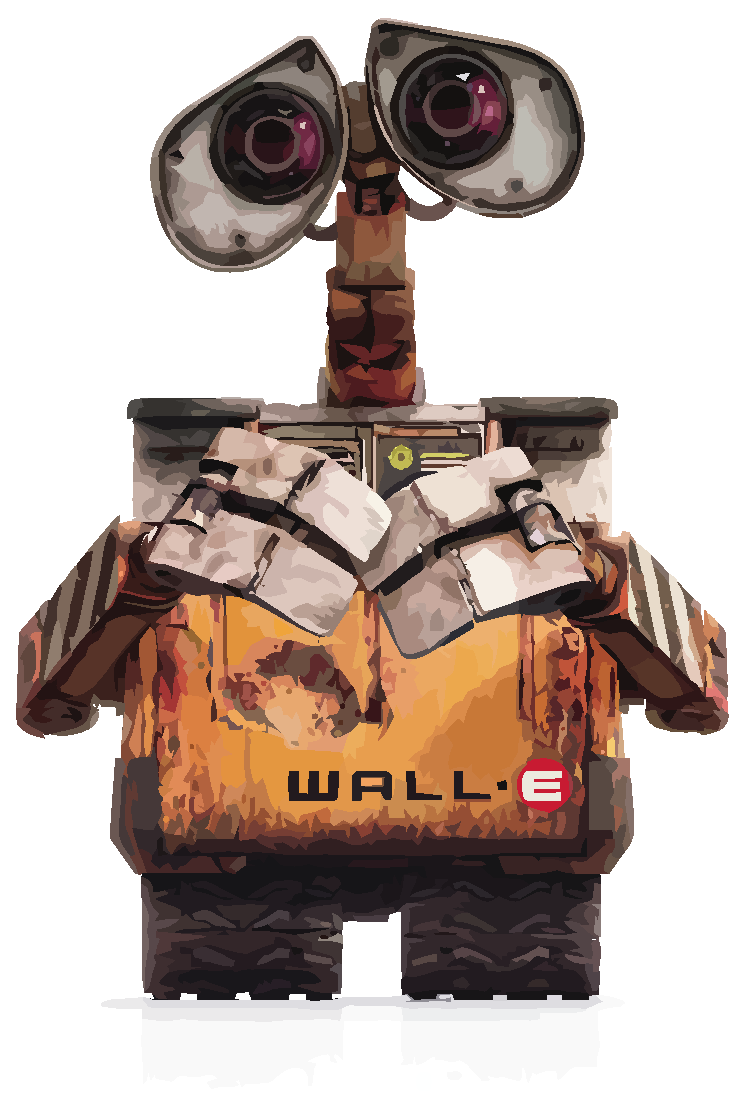
\includegraphics[width=\textwidth]{WallE}
    \caption{Wall-E}
    \label{fig:WallE}
  \end{subfigure}             
  \begin{subfigure}[b]{0.3\textwidth}
    
\includegraphics[width=\textwidth]{minion}
    \caption{Minions}
    \label{fig:Minnion}
  \end{subfigure}
  \caption{Best Animations}
  \label{fig:animations}
\end{figure}


\end{landscape}

%!TEX root = ../thesis.tex
%*******************************************************************************
%****************************** Third Chapter **********************************
%*******************************************************************************
\chapter{Causal Abstractions}

% **************************** Define Graphics Path **************************
\ifpdf
    \graphicspath{{Chapter3/Figs/Raster/}{Chapter3/Figs/PDF/}{Chapter3/Figs/}}
\else
    \graphicspath{{Chapter3/Figs/Vector/}{Chapter3/Figs/}}
\fi

This chapter is based on the paper \emph{Causal Consistency of Structural Equation Models} published at UAI 2017.


%
%
%\begin{abstract}
%Complex systems can be modelled at various levels of detail.
%Ideally, causal models of the same system should be consistent with one another in the sense that they agree in their predictions of the effects of interventions.
%We formalise this notion of consistency in the case of Structural Equation Models (SEMs) by introducing \emph{exact transformations} between SEMs.
%This provides a general language to consider, for instance, the different levels of description in the following three scenarios:
%(a)~models with large numbers of variables versus models in which the `irrelevant' or unobservable variables have been marginalised out;
%(b)~micro-level models versus macro-level models in which the macro-variables are aggregate features of the micro-variables;
%(c)~dynamical time series models versus models of their stationary behaviour.
%Our analysis stresses the importance of well specified interventions in the causal modelling process and sheds light on the interpretation of cyclic SEMs.
%\end{abstract}





\section{Introduction}


Physical systems or processes in the real world are complex and can be understood at various levels of detail.
For instance, a gas in a volume consists of a large number of molecules.
But instead of modelling the motions of each particle individually (micro-level), we may choose to consider macroscopic properties of their motions such as temperature and pressure.
Our decision to use such macroscopic properties is first necessitated by practical considerations.
Indeed, for all but extremely simple cases, making a measurement of all the individual molecules is practically impossible and our resources insufficient for modelling the ${\sim}10^{22}$ particles present per litre of ideal gas.
Furthermore, the decision for a macroscopic description level is also a pragmatic one: if we only wish to reason about temperature and pressure, a model of $10^{22}$ particles is ill-suited.

Statistical physics explains how higher-level concepts such as temperature and pressure arise as statistical properties of a system of a large number of particles, justifying the use of a macro-level model as a useful transformation of the micro-level model~\citep{Balian}.
However, in many cases aggregate or indirect measurements of a complex system form the basis of a macroscopic description of the system, with little theory to explain whether this is justified or how the micro- and macro-descriptions stand in relation to each other.

Due to deliberate modelling choice or the limited ability to observe a system, differing levels of model descriptions are ubiquitous and occur, amongst possibly others, in the following three settings:
\vspace{-.5em}
\begin{itemize}[noitemsep]
    \item[(a)] Models with large numbers of variables versus models in which the `irrelevant' or unobservable variables have been marginalised out \citep{bongers2016structural}; e.\,g.\ modelling blood cholesterol levels and risk of heart disease while ignoring other blood chemicals or external factors such as stress.

    \item[(b)] Micro-level models versus macro-level models in which the macro-variables are aggregate features of the micro-variables \citep{simon1961aggregation,iwasaki1994causality,hoel2013quantifying,chalupka2015visual,chalupka2016multi}; e.\,g.\ instead of modelling the brain as consisting of $100$ billion neurons it can be modelled as averaged neuronal activity in distinct functional brain regions.

    \item[(c)] Dynamical time series models versus models of their stationary behaviour \citep{fisher1970correspondence,iwasaki1994causality,dash2001caveats,lacerda2012discovering,mooij2013ode,mooij2013cyclic}; e.\,g.\ modelling only the final ratios of reactants and products of a time evolving chemical reaction.
\end{itemize}
\vspace{-.5em}
In the context of causal modelling, such differing model levels  should be consistent with one another in the sense that they agree in their predictions of the effects of interventions. The particular causal models we focus on in this paper are Structural Equation Models (SEMs, Section~\ref{sec:SEMs}, Section~\ref{sec:sem-for-causal-modelling}) \citep{spirtes2000causation,pearl2009causality}.

In Section~\ref{sec:sem-transformation}, we introduce the notion of an exact transformation between two SEMs, providing us with a general framework to evaluate when two models can be thought of as causal descriptions of the same system.
An important novel idea of this paper is to explicitly make use of a natural ordering on the set of interventions.
On a high level, if an SEM can be viewed as an exact transformation of another SEM, we are provided with an explicit correspondence between the two models in such a way that causal reasoning on both levels is consistent.
We discuss this notion of consistency in detail in Sections~\ref{subsec:causal-interpretation-transformation} and~\ref{sec:wrong}.

In Section~\ref{sec:example-transformations} we apply this mathematical framework and prove the exactness of transformations belonging to each of the three categories listed above, with practical implications for the following questions in causal modelling:
When can we model only a subsystem of a more complex system?
When does a micro-level system admit a causal description in terms of macro-level features?
How do cyclic SEMs arise?
The fact that these distinct problems can all be considered using the language of transformations between SEMs demonstrates the generality of our approach.
We close in Section~\ref{sec:questions} with a discussion.




\subsection{A historical motivation: Cholesterol and Heart Disease}\label{sec:cholesterol}

\begin{figure}
\begin{subfigure}{.45\linewidth}
\center\
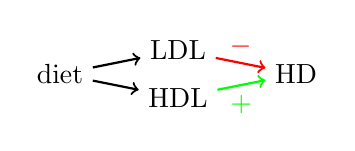
\begin{tikzpicture}
\node (d1) at(0,0.0) {diet};
\node (LDL) at(1.5,0.3) {LDL};
\node (HDL) at(1.5,-0.3) {HDL};
\node (HD) at(3,0) {HD};

\draw[->,thick] (d1) -- (HDL);
\draw[->,thick] (d1) -- (LDL);
\draw[->,red,thick] (LDL) -- node[above,yshift=-1] {$-$} (HD);
\draw[->,green,thick] (HDL) -- node[below] {$+$} (HD);
\end{tikzpicture}
\caption{}\label{fig:cholesterol:b}
\end{subfigure}
%
\hfill
%
\begin{subfigure}{.45\linewidth}
\center\
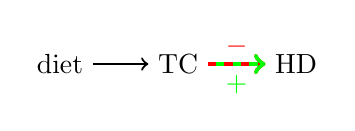
\begin{tikzpicture}
\node (d1) at(0,0.) {diet};
\node (LHDL) at(1.5,0) {TC};
\node (HD) at(3,0) {HD};

\draw[->,thick] (d1) -- (LHDL);
\draw[->,red,dash pattern= on 3pt off 3pt,ultra thick] (LHDL) -- node[above,yshift=-1] {$-$} (HD);
\draw[->,green,dash pattern= on 3pt off 3pt,dash phase=3pt,ultra thick] (LHDL) -- node[below] {$+$} (HD);
\end{tikzpicture}
\caption{}\label{fig:cholesterol:a}
\end{subfigure}
%
\caption{As illustrated by~(a), the current consensus is that LDL (resp.\ HDL) has a negative (resp.\ positive) effect on heart disease (HD). Considering TC = LDL + HDL to be a causal variable as in~(b) leads to problems: two diets promoting raised LDL levels and raised HDL levels have the same effect on TC but opposite effects on heart disease. Hence different studies come to contradictory conclusions about the effect of TC on heart disease.}
\label{fig:cholesterol}
\end{figure}


In the following we give an example of the problems that can arise when there exists no consistent correspondence between two causal models, i.\,e.\ neither model can be viewed as an exact transformation of the other. This example falls into category (b) of the differing model levels listed above and was used by~\cite{spirtes2004causal} to illustrate problems in the causal modelling process.

Historically, the level of total cholesterol in the blood (TC) was thought to be an important variable in determining risk of heart disease (HD).
To investigate this, different experiments were carried out in which patients were assigned to different diets in order to raise or lower TC\@.
Conflicting evidence was found by different experiments: some found that higher TC had the effect of lowering HD, while others found the opposite (cf.\ Figure~\ref{fig:cholesterol:a}) \citep{truswell2010cholesterol,steinberg2011cholesterol}.

From our point of view, this problem (seemingly conflicting studies) arose from trying to perform an `invalid' transformation of the `true' underlying model (cf.\ Figure~\ref{fig:cholesterol:b}).
According to the American Heart Association, the current scientific consensus is that the two types of blood cholesterol, low-density lipoprotein (LDL) and high-density lipoprotein (HDL), have a negative and positive effect on HD respectively.
Assigning diets that raise LDL or HDL both raise TC but have different effects on HD\@.
It is therefore not possible to transform the model in Figure~\ref{fig:cholesterol:b} into the model in Figure~\ref{fig:cholesterol:a} without leading to conflict:
in order to reason about the causes of HD we need to consider the variables LDL and HDL separately.





\section{Structural Equation Models}\label{sec:SEMs}

SEMs are a widely used framework in causal modelling, with applications in neuroscience, economics and the social sciences \citep{pearl2009causality,bollen2014structural}. In this section we introduce them as an abstract mathematical object; in Section~\ref{sec:sem-for-causal-modelling} we describe their use as a causal modelling tool.
Readers already familiar with SEMs should note that our definition is more general and deviates from the standard definition of SEMs in the following ways: we do not require that all possible perfect interventions be modelled; we do not assume independence of exogenous variables;\footnote{Exogenous variables are also referred to as \emph{noise variables} in the literature. Our relaxation of the assumption of independent exogenous variables means our models may be considered a type of semi-Markovian causal model.} and we do not require acyclicity.
%

\begin{definition}[Structural Equation Model (SEM)]
    Let $\indexset_X$ be an index set.
    An SEM $\mathcal{M}_X$ over  variables ${X = (X_i : i\in\indexset_X )}$ taking value in $\mathcal{X}$ is a triple $\left(\mathcal{S}_X, \mathcal{I}_X, \mathbb{P}_{E} \right)$ where
    \vspace{-.5em}
    \begin{itemize}[noitemsep]
        \item $\mathcal{S}_X$ is a set of structural equations, i.\,e.\ it is a set of equations $X_i = f_i\left( X , E_i \right)\ $ for $i \in \indexset_X$;
        \item ($\mathcal{I}_X, \leq_X)$ is a subset of all perfect interventions equipped with a natural partial ordering (see below), i.\,e.\ it is an index set where each index corresponds to a particular perfect intervention on some of the $X$ variables;
        \item $\mathbb{P}_{E}$ is a distribution over the exogenous variables $E = ( E_i : i\in\indexset_X)$;
        \item with $\mathbb{P}_E$-probability one, under any intervention ${i \in \mathcal{I}_X}$ there is a unique solution $x\in\mathcal{X}$ to the intervened structural equations. This ensures that for any intervention ${i \in \mathcal{I}_X}$, $\mathcal{M}_X$ induces a well-defined distribution over $\mathcal{X}$.%
\footnote{That is, with probability one over the exogenous variables $E$, for each draw $E=e$ there exists a unique value $x\in \mathcal{X}$ such that $e$ and $x$ satisfy the intervened structural equations. The distribution of $E$ in conjunction with $\mathcal{S}_X$ then implies a distribution over $\mathcal{X}$ for each intervention $i \in \mathcal{I}_X$ via these unique solutions.
If the SEM is acyclic, this is always satisfied; we impose this condition because we also consider \emph{cyclic} SEMs \cite{bongers2016structural}.}
    \end{itemize}
    \vspace{-.5em}
\end{definition}

In an SEM, each $X_i$ is a function of the $X$-variables and the exogenous variable $E_i$.
In this mathematical model, a perfect intervention on a single variable $\doop(X_i=x_i)$ is realised by replacing the structural equation for variable $X_i$ in $\mathcal{S}_X$ with $X_i = x_i$.
Perfect interventions on multiple variables, e.g. $\doop(X_i=x_i, X_j=x_j)$, are similarly realised by replacing the structural equations for each variable individually.
Elements of $\mathcal{I}_X$ correspond to perfectly intervening on a subset of the $X$ variables, setting them to some particular combination of values.

$\mathcal{I}_X$ has a natural partial ordering in which, for interventions ${i, j \in \mathcal{I}_X}$, ${i\leq_X j}$ if and only if $i$ intervenes on a subset of the variables that $j$ intervenes on and sets them equal to the same values as $j$.
For example, ${\doop(X_i=x_i) \leq_X \doop(X_i=x_i, X_j=x_j)}$.\footnote{Informally, this means that $j$ can be performed after $i$ without having to change or undo any of the changes to the structural equations made by $i$.
Not all pairs of elements must be comparable: for instance, if $i= \doop(X_1=x_1)$ and $j = \doop(X_2=x_2)$, then neither $i\leq_X j$ nor $j \leq_X i$.} The observation that this structure is important is a contribution of this paper. We make crucial use of it in the next section.

The purpose of the following example is to illustrate how SEMs are written in our notation and to provide and example of a restricted set of interventions $\mathcal{I}_X$.

\begin{example}\label{example1}
Consider the following SEM defined over the variables $\{ B_1,B_2,L \}$
%
\begin{align*}
\mathcal{S}_X = \big\{ & B_1 = E_1,\ B_2 = E_2,\ L = \operatorname{OR}(B_1,B_2,E_3) \big\} \\
%
\mathcal{I}_X = \big\{ & \nulli,\ \doop(B_1=0),\ \doop(B_2=0),\\
& \doop(B_1=0,B_2=0) \big\}, \\
%
\{ E_1,E_2,E_3 \} & \overset{\text{iid}}{\sim} \mathrm{Bernoulli}(0.5)
\end{align*}
%
where by the element $\nulli \in \mathcal{I}$ we denote the null-intervention corresponding to the unintervened SEM\@.
\end{example}

\section{SEMs for Causal Modelling}\label{sec:sem-for-causal-modelling}

In addition to being abstract mathematical objects, SEMs are used in causal modelling to describe distributions of variables and how they change under interventions \citep{pearl2009causality}.
The $\doop$-interventions as abstract manipulations of SEMs are understood as corresponding to actual (or potentially only hypothetical) physical implementations in the real world, i.\,e.\ the model is `rooted in reality'.
For instance, if a binary variable $B_1$ in an SEM reflects whether a light bulb is emitting light, then $\doop(B_1=0)$ could be achieved by flipping the light switch or by removing the light bulb.

The SEM in Example~\ref{example1} could be thought of as a simple causal model of two light bulbs $B_1$ and $B_2$ and the presence of light $L$ in a room with a window.
Suppose that we have no access to the light switch and there are no curtains in the room but that we can intervene by removing the light bulbs.
We can model this restricted set of interventions by $\mathcal{I}_X$, i.\,e.\ the $\doop$-intervention on the SEM side ${\doop(B_1=0)}$  corresponds to removing the light bulb $B_1$.

The partial ordering of $\mathcal{I}_X$ corresponds to the ability to compose physical implementations of interventions. The fact that we can first remove light bulb $B_1$ (${\doop(B_1=0)}$) and then afterwards remove light bulb $B_2$ (resulting in the combined intervention ${\doop(B_1=0, B_2=0)}$)  is reflected in the partial ordering via the relation ${\doop(B_1=0) \leq_X \doop(B_1=0,B_2=0)}$.
%

\section{Transformations between SEMs}\label{sec:sem-transformation}

We now work towards our definition of an exact transformation between SEMs\@.
Our core idea is to analyse the correspondence between different levels of modelling by considering one model to be a transformation of the other.
We discuss in Section~\ref{subsec:causal-interpretation-transformation} how causal reasoning in two SEMs relate when one SEM can be viewed as an exact transformation of the other and in Section~\ref{sec:wrong} we illustrate what can go wrong when this is not the case.

\subsection{Distributions implied by an SEM}

Usually, a statistical model implies a single joint distribution over all variables once its parameters are fixed.
SEMs are different in that, once the parameters are fixed, an SEM implies a family of joint distributions over the random variables, one for each intervention.
That is, for each intervention $i \in \mathcal{I}_X$, the SEM $\mathcal{M}_X$ defines a distribution over $\mathcal{X}$ which we denote by $\mathbb{P}_X^{\doop(i)}$.
Throughout, we will denote the null-intervention corresponding to the unintervened setting by $\nulli\in \mathcal{I}_X$ .
We can write the poset of all distributions implied by the SEM $\mathcal{M}_X$ as
\[\mathcal{P}_X := \left( \left\{ \mathbb{P}_X^{\doop(i)} \enspace : \enspace i \in \mathcal{I}_X \right\}, \leq_X \right) \]
where $\leq_X$ is the partial ordering inherited from $\mathcal{I}_X$, i.\,e.\ ${\mathbb{P}_X^{\doop(i)} \leq_X \mathbb{P}_X^{\doop(j)} \iff i \leq_X j}$.%
\footnote{More formally, one would need to define $\mathcal{P}_X$ to be the poset of \emph{tuples} $\left(i, \mathbb{P}_X^{\doop(i)}\right)$ to avoid problems in the case that $\mathbb{P}_X^{\doop(i)} = \mathbb{P}_X^{\doop(j)}$ for some $i\not=_X j$. Doing so would not require a change to Definition~3 or affect the further results of this paper. To avoid notational burden in our exposition, we omit this treatment.}

Note that $\mathcal{P}_X$ contains all of the information in $\mathcal{M}_X$ about the different distributions implied by the SEM and, importantly, how they are related via the interventions.%
\footnote{For example, the distribution over the variables $X$ in the observational setting, $\mathbb{P}_X^\nulli$, changes to $\mathbb{P}_X^{\doop(i)}$ if we implement the intervention ${\doop(i)}$, and the partial ordering contains all information about which interventions can be composed.}


\subsection{Transformations of random variables}

Suppose we have a function ${\tau: \mathcal{X} \to \mathcal{Y}}$ which maps the variables of the SEM $\mathcal{M}_X$ to another space $\mathcal{Y}$.
Observe that since $X$ is a random variable, $\tau(X)$ is also a random variable.
For any distribution $\mathbb{P}_X$ on $\mathcal{X}$ we thus obtain the distribution of the variable $\tau(X)$ on $\mathcal{Y}$ as $\mathbb{P}_{\tau(X)} = \tau\left(\mathbb{P}_X\right)$ via the push-forward measure.

In particular, for each intervention $i \in \mathcal{I}_X$ we can define the induced distribution $\mathbb{P}_{\tau(X)}^{i} = \tau\left(\mathbb{P}_X^{\doop(i)}\right)$.
We can write the poset of distributions on $\mathcal{Y}$ that are induced by the original SEM $\mathcal{M}_X$ and the transformation $\tau$ as
\[\mathcal{P}_{\tau(X)} := \left( \left\{ \mathbb{P}_{\tau(X)}^{i} \enspace : \enspace i \in \mathcal{I}_X \right\}, \leq_X \right) \]
where $\leq_X$ is the partial ordering inherited from $\mathcal{P}_X$ (and in turn from $\mathcal{I}_X$).

$\mathcal{P}_{\tau(X)}$ is just a structured collection of distributions over $\mathcal{Y}$, indexed by interventions $\mathcal{I}_X$ on the $\mathcal{X}$-level; importantly, the indices are \emph{not} interventions on the $\mathcal{Y}$-level.

\subsection{Exact Transformations between SEMs}\label{sec:exact_transformation_sem}

Although $\mathcal{P}_{\tau(X)}$ is a poset of distributions over $\mathcal{Y}$, there does not necessarily exist an SEM $\mathcal{M}_Y$ over $\mathcal{Y}$ that implies it.
For instance, if there is some intervention ${i \in \mathcal{I}_X \setminus \{ \nulli \}}$ such that none of the variables $Y_i$ is constant under the distribution $\mathbb{P}_{\tau(X)}^{i}$, then $\mathbb{P}_{\tau(X)}^{i}$ could not possibly be expressed as arising from a $\doop$-intervention $j\in \mathcal{I}_Y \setminus \{\nulli\}$ in any SEM over~$\mathcal{Y}$.\footnote{This problem is elaborated upon in~\cite{eberhardt2016green}.}

The case in which there \emph{does} exist an SEM $\mathcal{M}_Y$ that implies $\mathcal{P}_{\tau(X)}$ is special, motivating our main definition.

\begin{definition}[Exact Transformations between SEMs]\label{def:exacttrafos}
Let $\mathcal{M}_X$ and $\mathcal{M}_Y$ be SEMs and $\tau: \mathcal{X} \to \mathcal{Y}$ be a function.
We say $\mathcal{M}_Y$ is an \emph{exact}  $\tau$-transformation of $\mathcal{M}_X$ if there exists a \emph{surjective order-preserving} map $\omega:\mathcal{I}_X\rightarrow \mathcal{I}_Y$ such that
\[ \mathbb{P}_{\tau(X)}^{i} = \mathbb{P}_Y^{\doop(\omega(i))} \quad \forall i \in \mathcal{I}_X \]
where $\mathbb{P}_{\tau(X)}^{i}$ is the distribution of the $\mathcal{Y}$-valued random variable $\tau(X)$ with $X \sim \mathbb{P}_X^{\doop(i)}$.
\end{definition}

Order-preserving means that ${i \leq_X j \implies \omega(i) \leq_Y \omega(j)}$.
It is important that the converse need not in general hold as this would imply that $\omega$ is injective,%
\footnote{Since ${\omega(i)=\omega(j) \iff \left(\omega(i) \leq_Y \omega(j)\right) \land \left(\omega(j) \leq_Y \omega(i)\right)}$, which, if the converse held, would imply that $\left(i \leq_X j\right) \land \left(j \leq_X i\right)$, which is equivalent to $i=j$.}
and hence also bijective.
This would constrain the ways in which $\mathcal{M}_Y$ can be `simpler' than $\mathcal{M}_X$.\footnote{For instance, if it were necessary that $\omega$ be bijective, Theorems~\ref{theorem:childless} and \ref{theorem:micro-macro} would not hold.}
That $\omega$ is surjective ensures that for any $\doop$-intervention $j \in \mathcal{I}_Y$ on $\mathcal{M}_Y$ there is at least one corresponding intervention on the $\mathcal{M}_X$ level, namely an element of $\omega^{-1}(\{j\}) \subseteq \mathcal{I}_X$.
The following two results follow immediately from the definition (cf.\ proofs in Appendix~\ref{first_properties:appendix}).

\begin{lemma}\label{lemma:elementary}
The identity mapping and permuting the labels of variables are both exact transformations.
\end{lemma}

This is a good sanity check; it would be problematic if this were not the case and the labelling of our variables mattered. Similarly, compositions of exact transformations are also exact.

\begin{lemma}[Transitivity of exact transformations]\label{theorem:transitivity}
    If $\mathcal{M}_Z$ is an exact $\tau_{ZY}$-transformation of $\mathcal{M}_Y$ and $\mathcal{M}_Y$ is an exact $\tau_{YX}$-transformation of $\mathcal{M}_X$, then $\mathcal{M}_Z$ is an exact $(\tau_{ZY}\circ\tau_{YX})$-transformation of $\mathcal{M}_X$.
\end{lemma}

The following theorem is a consequence of the fact that $\omega$ is order-preserving. This is a mathematical formalisation of the sense in which an exact transformation preserves causal reasoning, which will be elaborated upon in the next subsection.


\begin{theorem}[Causal consistency under exact transformations]\label{lemma:commuting}
Suppose that  $\mathcal{M}_Y$ is an exact $\tau$-transformation of $\mathcal{M}_X$ and $\omega$ is a corresponding surjective order-preserving mapping between interventions. Let $i,j \in \mathcal{I}_X$ be interventions such that $i\leq_X j$.
Then the following diagram commutes:\\
\begin{tikzpicture}[thick, every node/.style = {circle, minimum size=.5cm}]

{
  \node[draw=none](Px) {$\mathbb{P}_X$};
  \node[draw=none, right of=Px, xshift=2cm](PxInt) {$\mathbb{P}_X^{\doop(i)}$};
  \node[draw=none, right of=PxInt, xshift=2cm](PxInt2) {$\mathbb{P}_X^{\doop(j)}$};

  \node[draw=none, below of=Px, yshift=-1.5cm](Py) {$\mathbb{P}_Y$};
  \node[draw=none, right of=Py, xshift=2cm](PyInt) {$\mathbb{P}_Y^{\doop(\omega(i))}$};
  \node[draw=none, right of=PyInt, xshift=2cm](PyInt2) {$\mathbb{P}_Y^{\doop(\omega(j))}$};

  \draw[-{Latex[length=2mm,width=2mm]}](Px)--(Py);
  \draw[-{Latex[length=2mm,width=2mm]}](Px)--(PxInt);
  \draw[-{Latex[length=2mm,width=2mm]}](Py)--(PyInt);
  \draw[-{Latex[length=2mm,width=2mm]}](PxInt)--(PyInt);
  \draw[-{Latex[length=2mm,width=2mm]}](PxInt)--(PxInt2);
  \draw[-{Latex[length=2mm,width=2mm]}](PyInt)--(PyInt2);
  \draw[-{Latex[length=2mm,width=2mm]}](PxInt2)--(PyInt2);

  \node[draw=none, yshift=0.5cm](xInt) at ($(Px)!0.5!(PxInt)$){$\doop(i)$};
  \node[draw=none, yshift=0.5cm](xInt2) at ($(PxInt)!0.5!(PxInt2)$){$\doop(j)$};
  \node[draw=none, yshift=0.5cm](yInt) at ($(Py)!0.5!(PyInt)$){$\doop(\omega(i))$};
  \node[draw=none, yshift=0.5cm](yInt2) at ($(PyInt)!0.5!(PyInt2)$){$\doop(\omega(j))$};
  \node[draw=none, xshift=-0.5cm](tau) at ($(Px)!0.5!(Py)$){$\tau$};
  \node[draw=none, xshift=0.5cm](tauInt) at ($(PxInt)!0.5!(PyInt)$){$\tau$};
  \node[draw=none, xshift=0.5cm](tauInt2) at ($(PxInt2)!0.5!(PyInt2)$){$\tau$};
}
\end{tikzpicture}
\end{theorem}

\begin{proof}
Let $i,j\in\mathcal{I}_X$ be interventions with $i\leq_X j$.
The commutativity of the left square of the diagram follows immediately from the definition of an exact transformation.
It remains to be shown that the right square of the diagram commutes.
By definition we have that $\tau\left(\mathbb{P}_X^{\doop(i)}\right) = \mathbb{P}_Y^{\doop(\omega(i))}$ and $\tau\left(\mathbb{P}_X^{\doop(j)}\right) = \mathbb{P}_Y^{\doop(\omega(j))}$.
Thus, we only have to show that ${\mathbb{P}_Y^{\doop(\omega(i))} \leq_Y \mathbb{P}_Y^{\doop(\omega(j))}}$ as elements of $\mathcal{P}_Y$, i.\,e.\ that the arrow ${\mathbb{P}_Y^{\doop(\omega(i))} \xrightarrow{\doop(\omega(j))} \mathbb{P}_Y^{\doop(\omega(j))}}$ exists.
This follows from the order-preservingness of $\omega$.
\end{proof}

\subsection{Causal Interpretation of Exact Transformations}\label{subsec:causal-interpretation-transformation}

The notion of an exact transformation between SEMs was motivated by the desire to analyse the correspondence between two causal models describing the same system at different levels of detail.
The purpose of this section is to show that if one SEM can be viewed as an exact transformation of the other, then both can sensibly be thought of as causal models of the same system. In the following, we assume that $\mathcal{M}_Y$ is an exact $\tau$-transformation of $\mathcal{M}_X$ with $\omega$ the corresponding map between interventions.

Surjectivity of $\omega$ ensures that any intervention in $\mathcal{I}_Y$ can be viewed as an $\mathcal{M}_Y$-level representative of some intervention on the $\mathcal{M}_X$-level. Consequently, if $\doop$-interventions on the $\mathcal{M}_X$-level are in correspondence with physical implementations, then surjectivity of $\omega$ ensures that $\doop$-interventions on the $\mathcal{M}_Y$-level have at least one corresponding physical implementation, i.\,e.\ if $\mathcal{M}_X$ is `rooted in reality', then so is $\mathcal{M}_Y$.

Commutativity of the left hand part of the diagram ensures that the effects of interventions are consistently modelled by $\mathcal{M}_X$ and $\mathcal{M}_Y$.
Suppose we want to reason about the effects on the $\mathcal{M}_Y$-level caused by the intervention $j \in \mathcal{I}_Y$.
For example, we may wish to reason about how the temperature and pressure of a volume of gaseous particles is affected by being heated.
We could perform this reasoning by considering any corresponding $\mathcal{M}_X$-level intervention $i \in \omega^{-1}(\{j\})$ and considering the distribution this implies over $\mathcal{Y}$ via $\tau$.
In our example, this would correspond to considering how heating the volume of gas could be modelled by changing the motions of all the gaseous particles and then computing the temperature and pressure of the volume of particles.
Commutativity of the left hand part of the diagram implies that $\mathcal{M}_X$ and $\mathcal{M}_Y$ are consistent in the sense that $\mathcal{M}_Y$ allows us to immediately reason about the effect of the intervention $j\in\mathcal{I}_Y$ while being equivalent to performing the steps above.
That is, we can reason directly about temperature and pressure when heating a volume of gas without having to perform the intermediate steps that involve the microscopic description of the system.

Commutativity of the right hand side of the diagram ensures that once an intervention that fixes a subset of the variables has been performed, we can still consistently reason about the effects of further interventions on the remaining variables in $\mathcal{M}_X$ and $\mathcal{M}_Y$.
Furthermore, it ensures that compositionality of $\doop$-interventions on the $\mathcal{M}_X$-level carries over to the $\mathcal{M}_Y$-level, i.\,e.\ if the intervention $j$ on the $\mathcal{M}_X$-level can be performed additionally to the intervention $i$ in $\mathcal{M}_X$---that is, $i\leq_X j$---, then the same is true of their representations in $\mathcal{M}_Y$.

If $\mathcal{M}_X$ and $\mathcal{M}_Y$ are models of the same system and it has been established that $\mathcal{M}_Y$ is an exact $\tau$-transformation of $\mathcal{M}_X$ for some mapping $\tau$, then the commutativity of the whole diagram in Theorem~\ref{lemma:commuting} ensures that they are causally consistent with one another in the sense described in the preceding paragraphs.
If we wish to reason about the effects of interventions on the $\mathcal{Y}$-variables then it suffices to use the model $\mathcal{M}_Y$, rather than the (possibly more complex) model $\mathcal{M}_X$.
In particular, this means that we can view the $\mathcal{Y}$-variables as causal entities, rather than only functions of underlying `truly' causal entities.
Only if this is the case, causal statements such as `raising temperature increases pressure' or `LDL causes heart disease' are meaningful.

\subsection{What can go wrong when a transformation is not exact?}\label{sec:wrong}

In the previous section we argued that our definition of exact transformations between SEMs is a sensible formalisation of causal consistency.
In this section we will try to give the reader an intuition for why weakening the conditions of our definition would be problematic.
In particular we focus on the requirement that $\omega$ be order-preserving, which we view as one of the core ideas of our paper.

The requirement that $\omega$ be surjective is, as discussed above, required so that all interventions on the $\mathcal{M}_Y$-level have a corresponding intervention on the $\mathcal{M}_X$-level.
If we were to only require that $\omega$ be surjective (but not order-preserving), the observational distribution of $\mathcal{M}_X$ may be mapped to an interventional distribution of $\mathcal{M}_Y$, as illustrated by the following example (cf.\ Figure~\ref{fig:wrong-example} for an illustration).

\begin{figure}
\begin{subfigure}{.45\linewidth}
\center\
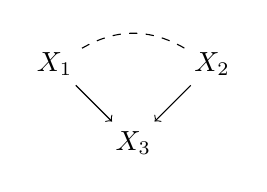
\begin{tikzpicture}
\node (x1) at(0,0) {$X_1$};
\node (x2) at(2,0) {$X_2$};
\node (x3) at(1,-1) {$X_3$};

\draw[->] (x1) -- (x3);
\draw[->] (x2) -- (x3);
\draw[dashed] (x1) to [bend left] (x2);
\end{tikzpicture}
\caption{SEM $\mathcal{M}_X$}
\end{subfigure}
%
\hfill
%
\begin{subfigure}{.45\linewidth}
\center\
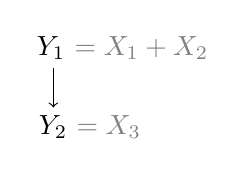
\begin{tikzpicture}
\node (y1) at(0,0) {$Y_1\ {\color{gray}= X_1+X_2}$};
\node (y2) at(-.415,-1) {$Y_2\ {\color{gray}= X_3}$};

\draw[->] (-.88,-.25) -- (-.88,-.75);
\end{tikzpicture}
\caption{SEM $\mathcal{M}_Y$}
\end{subfigure}
%
\caption{Graphical illustration of parent-child relationships for the examples in Section~\ref{sec:wrong}. The micro-level model $\mathcal{M}_X$ depicted in (a) is to be transformed into the macro-level model $\mathcal{M}_Y$ depicted in (b) which is a coarser descriptions as in it only considers the sum of $X_1$ and $X_2$. In Section~\ref{sec:wrong} we give examples of what can go wrong if the transformation is not exact.}
\label{fig:wrong-example}
\end{figure}

\begin{example}\label{example:wrong1}
Consider the SEM $\mathcal{M}_X=\{\mathcal{S}_X , \mathcal{I}_X, \mathbb{P}_E\}$ over $\mathcal{X}=\mathbb{R}^3$ where
%
\begin{align*}
\mathcal{S}_X = \big\{ & X_1 = E_1,\ X_2 = E_2,\ X_3 = X_1 + X_2 + E_3 \big\} \\
%
\mathcal{I}_X = \big\{ & \nulli,\ \doop(X_2=0),\ \doop(X_1=0,\, X_2=0)\big\}, \\
%
E_1 & \sim \mathbb{P}_{E_1},\ \,  E_2 = - E_1, \  \, E_3 \sim \mathbb{P}_{E_3}
\end{align*}
%
where $\mathbb{P}_{E_1}$ and $\mathbb{P}_{E_3}$ are arbitrary distributions.
Let ${\tau:\mathcal{X}\to\mathcal{Y}=\mathbb{R}^2}$ be the mapping such that
\begin{align*}
\tau\begin{pmatrix} x_1, x_2, x_3 \end{pmatrix}
= \begin{pmatrix} y_1, y_2\end{pmatrix}
= \begin{pmatrix} x_1 + x_2, x_3\end{pmatrix}
\end{align*}
%
Let $\mathcal{M}_Y =\{\mathcal{S}_Y , \mathcal{I}_Y, \mathbb{P}_F\}$ be an SEM over $\mathcal{Y}$ with
%
\begin{align*}
\mathcal{S}_Y = \big\{ & Y_1 = F_1,\ Y_2 = Y_1 + F_2 \big\} \\
%
\mathcal{I}_Y = \big\{ & \nulli,\ \doop(Y_1=0) \big\}, \\
%
F_1 \sim \mathbb{P}_{E_1},&  \  \, F_2 \sim \mathbb{P}_{E_3}
\end{align*}
%
Let ${\omega:\mathcal{I}_X \to \mathcal{I}_Y}$ be defined by
%
\begin{align*}
\omega: \begin{cases}
\nulli &\mapsto \doop(Y_1=0) \\
\doop(X_2=0) &\mapsto \nulli \\
\doop(X_1=0,\, X_2=0) &\mapsto \doop(Y_1=0) \\
\end{cases}
\end{align*}
%
Then it is true that ${\mathbb{P}_{\tau(X)}^{i} = \mathbb{P}_Y^{\doop(\omega(i))}}$ for all  ${i \in \mathcal{I}_X }$, while $\omega$ is not order-preserving and $\omega(\nulli)\not = \nulli$.
\end{example}

If the SEMs in the above example were used to model the same system, it would be problematic that the observational setting of $\mathcal{M}_X$---a description of the system when not having physically performed any intervention---would correspond to an interventional setting in $\mathcal{M}_Y$, conversely suggesting that the system \emph{had} been intervened upon.

To avoid the above conflict, we could demand in addition to surjectivity that $\omega$ map the null intervention of $\mathcal{M}_X$ to the null intervention of $\mathcal{M}_Y$.
This additional assumption would ensure commutativity of the left-hand part of the diagram in Theorem~\ref{lemma:commuting}.
However, as the following example shows, this would not ensure that the right-hand part of the diagram commutes for all pairs of interventions ${i \leq_X j}$, since in this case the arrow from $\mathbb{P}_Y^{\doop(\omega(i))}$ to $\mathbb{P}_Y^{\doop(\omega(j))}$ may not exist.\footnote{By definition of the poset $\mathcal{P}_Y$, this arrow exists if and only if $\omega(i) \leq_Y \omega(j)$.}

\begin{example}\label{example:wrong2}
Let $\mathcal{X},\mathcal{Y}$ and $\tau$ be as in Example~\ref{example:wrong1}. Consider the SEM $\mathcal{M}_X=\{\mathcal{S}_X , \mathcal{I}_X, \mathbb{P}_E\}$ where
%
\begin{align*}
\mathcal{S}_X = \big\{ & X_1 = E_1,\ X_2 = E_2, \ X_3 = X_1 + X_2 + E_3 \big\} \\
%
\mathcal{I}_X = \big\{ & \nulli,\ \doop(X_2=0),\ \doop(X_1=0,\, X_2=0)\big\}, \\
%
E_1 & = 1,\ \,  E_2 \sim \mathbb{P}_{E_2}, \  \, E_3 \sim \mathbb{P}_{E_3}
\end{align*}
%
where $\mathbb{P}_{E_2}$ and $\mathbb{P}_{E_3}$ are arbitrary distributions.
%
Let $\mathcal{M}_Y =\{\mathcal{S}_Y , \mathcal{I}_Y, \mathbb{P}_F\}$ be the SEM over $\mathcal{Y}$ with
%
\begin{align*}
\mathcal{S}_Y = \big\{ & Y_1 =1+ F_1,\ Y_2 = Y_1 + F_2 \big\} \\
%
\mathcal{I}_Y = \big\{ & \nulli,\ \doop(Y_1=0),\ \doop(Y_1=1) \big\}, \\
%
F_1 &\sim \mathbb{P}_{E_2},  \  \, F_2 \sim \mathbb{P}_{E_3}
\end{align*}
%
Let ${\omega:\mathcal{I}_X \to \mathcal{I}_Y}$ be defined by
%
\begin{align*}
\omega: \begin{cases}
\nulli &\mapsto \nulli  \\
\doop(X_2=0) &\mapsto \doop(Y_1=1) \\
\doop(X_1=0,\, X_2=0) &\mapsto \doop(Y_1=0) \\
\end{cases}
\end{align*}
%
Then it is true that ${\mathbb{P}_{\tau(X)}^{i} = \mathbb{P}_Y^{\doop(\omega(i))}}$ for all ${i \in \mathcal{I}_X}$ and $\omega(\nulli)=\nulli$, although $\omega$ is not order-preserving.
\end{example}

If the above SEMs were used as models of the same system, they would not suffer from the problem illustrated in Example~\ref{example:wrong1}.
Suppose now, however, that we have performed the intervention $\doop(X_2=0)$ in $\mathcal{M}_X$, corresponding to the intervention $\doop(Y_1=1)$ in $\mathcal{M}_Y$.
If we wish to reason about the effect of the intervention $\doop(X_1=0,\, X_2=0)$ in $\mathcal{M}_X$, we run into a problem.
$\mathcal{M}_X$ suggests that $\doop(X_1=0,\, X_2=0)$ could be implemented by performing an additional action on top of $\doop(X_2=0)$.
In contrast, $\mathcal{M}_Y$ suggests that implementing the corresponding intervention $\doop(Y_1=0)$ would conflict with the already performed intervention $\doop(Y_1=1)$.
%

\section{Examples of exact transformations}\label{sec:example-transformations}

In the introduction we motivated the problem considered in this paper by listing three settings in which differing model levels naturally occur.
Having now introduced the notion of an exact transformation between SEMs, we provide in this section examples of exact transformations falling into each of these categories.
The fact that a single framework can be used to draw an explicit correspondence between differing model levels in each of these settings demonstrates the generality of our framework.

Observe that in each of the following examples, the particular set of interventions considered is important. If we were to allow larger sets of interventions $\mathcal{I}_X$ in the SEM $\mathcal{M}_X$, the transformations given would not be exact. This highlights the importance to the causal modelling process of carefully considering the set of interventions. All proofs are found in  the Appendix.






\subsection{Marginalisation of variables}\label{sec:basic_trafos}

In the following two Theorems we consider two operations that can be performed on SEMs, namely marginalisation of childless or non-intervened variables, and prove that these are exact transformations.
That is, an SEM can be simplified into an SEM with fewer variables by either of these operations without losing any causal content concerning the remaining variables.

Thus if the SEM $\mathcal{M}_Y$ can be obtained from another SEM $\mathcal{M}_X$ by successively performing the operations in the following theorems, then $\mathcal{M}_Y$ is an exact transformation of $\mathcal{M}_X$ and hence the two models are causally consistent.
This formally explains why we can sensibly consider causal models that focus on a subsystem $\mathcal{M}_Y$ of a more complex system $\mathcal{M}_X$ (cf.\ Figure~\ref{fig:SEM_marginalisation}).
For a measure-theoretic treatment of marginalisation in SEMs, see~\cite{bongers2016structural}.

\begin{theorem}[Marginalisation of childless variables]\label{theorem:childless}
Let $\mathcal{M}_X=(\mathcal{S}_X,\mathcal{I}_X,\mathbb{P}_E)$ be an SEM and suppose that ${\mathbb{I}_Z\subset\mathbb{I}_X}$ is a set of indices of variables with no children, i.\,e.\ if $i\in\mathbb{I}_Z$ then $X_i$ does not appear in the right-hand side of any structural equation in $\mathcal{S}_X$.
Let $\mathcal{Y}$ be the set in which $Y = \left( X_i: i\in\mathbb{I}_X\setminus \mathbb{I}_Z \right)$ takes value.
Then the transformation $\tau: \mathcal{X} \to \mathcal{Y}$ mapping
\begin{align*}
   \tau: \left( x_i: i\in\mathbb{I}_X \right) = x &\mapsto y = \left( x_i: i\in\mathbb{I}_X\setminus \mathbb{I}_Z \right)
\end{align*}
naturally gives rise to an SEM $\mathcal{M}_Y$ that is an exact $\tau$-transformation of $\mathcal{M}_X$, corresponding to marginalising out the childless variables $X_i$ for $i\in\mathbb{I}_Z$.
\end{theorem}




\begin{theorem}[Marginalisation of non-intervened variables]\label{theorem:never_intervened}
Let $\mathcal{M}_X=(\mathcal{S}_X,\mathcal{I}_X,\mathbb{P}_E)$ be an \emph{acyclic} SEM and suppose that ${\mathbb{I}_Z\subset\mathbb{I}_X}$ is a set of indices of variables that are not intervened upon by any intervention $i\in\mathcal{I}_X$.
Let $\mathcal{Y}$ be the set in which $Y = \left( X_i: i\in\mathbb{I}_X\setminus \mathbb{I}_Z \right)$ takes value.
Then the transformation $\tau: \mathcal{X} \to \mathcal{Y}$ mapping
\begin{align*}
   \tau: \left( x_i: i\in\mathbb{I}_X \right) = x &\mapsto y = \left( x_i: i\in\mathbb{I}_X\setminus \mathbb{I}_Z \right)
\end{align*}
naturally gives rise to an SEM $\mathcal{M}_Y$ that is an exact $\tau$-transformation of $\mathcal{M}_X$, corresponding to marginalising out the never-intervened-upon variables $X_i$ for $i\in\mathbb{I}_Z$.
\end{theorem}

The assumption of acyclicity made in Theorem~\ref{theorem:never_intervened} can be relaxed to allow marginalisation of non-intervened variables in cyclic SEMs, at the expense of extra technical conditions (see Section~3 of \cite{bongers2016structural}).


\begin{figure}
\center\
%
\begin{tikzpicture}

\node[keep] (X1) at(0,0) {$X_1$};
\node[keep] (X2) at(1.5,1.5) {$X_2$};
\node[keep] (X3) at(3,0) {$X_3$};

\node[drop1] (d1) at(4.5,.25) {};
\node[drop1] (d2) at(4.5,1.25) {};
\node[drop1] (d3) at(5,.75) {};

\draw[->,docolour] (X3) -- (d1);
\draw[->,docolour] (X2) -- (d2);
\draw[->,docolour] (d2) -- (d1);
\draw[->,docolour] (d1) -- (d3);
\draw[->,docolour] (d2) -- (d3);
\draw[->,docolour,dashed] (d1) -- (5,0);
\draw[->,docolour,dashed] (d2) -- (5,1.5);

\node[drop2a] (i12) at(.75,.75) {};
\node[drop2a] (i23) at(2.25,.75) {};
\node[drop2a] (i13a) at(1,0) {};
\node[drop2a] (i13b) at(2,0) {};

\draw[->] (X1) -- (i12) -- (X2);
\draw[->] (X2) -- (i23) -- (X3);
\draw[->] (X1) -- (i13a) -- (i13b) -- (X3);
\draw[->,docolour,dashed] (i13a) -- (1.25,-1);

\node[drop2b] (n1) at(-1.5,.5) {};
\node[drop2b] (n2) at(-1,1.5) {};
\node[drop2b] (n3) at(-1.75,1.25) {};

\draw[->,docolour] (n1) -- (X1);
\draw[->,docolour] (n3) -- (n1);
\draw[->,docolour] (n1) -- (n2);
\draw[->,docolour] (n3) -- (n2);
\draw[->,docolour,dashed] (-1.75,0) -- (n1);
\draw[->,docolour,dashed] (-1.75,2) -- (n2);
\draw[->,docolour,dashed] (-1,-.25) -- (X1);
\draw[->,docolour,dashed] (-.5,2.5) -- (X2);

\draw[dotted] (-.75,2.25) -- (3.75,2.25) -- (3.75,-.75) -- (-.75,-.75) -- (-.75,2.25);
\node (label) at(1.5,2.5) {subsystem $\mathcal{M}_Y$};
\node (label2) at(-1.75,-.75) {$\mathcal{M}_X$};

\end{tikzpicture}
%
\caption{Suppose that there is a complex model $\mathcal{M}_X$ but that we only wish to model the distribution over $X_1,X_2,X_3$ and how it changes under some interventions on $X_1,X_2,X_3$.
By Theorem~\ref{theorem:childless}, we can ignore downstream effects (\dropNode{drop1}) after grouping them together as one multivariate variable and by Theorem~\ref{theorem:never_intervened} we can ignore intermediate steps of complex mechanisms (\dropNode{drop2a}) and treat upstream causes as noise fluctuations (\dropNode{drop2b}).
That is, we can exactly transform the complex SEM $\mathcal{M}_X$ into a simpler model $\mathcal{M}_Y$ by marginalisation.
}
\label{fig:SEM_marginalisation}
\end{figure}


We remind the reader that our definition of an SEM does not require that the exogenous $E$-variables be independent. 
Theorem~\ref{theorem:never_intervened} would not hold if this restriction were made (which is usually the case in the literature); marginalising out a common parent node will in general result in its children having dependent exogenous variables.

\subsection{Micro- to macro-level}\label{subsection:micromacro}

Transformations from micro- to macro-levels may arise in situations in which the micro-level variables can be observed via a `coarse' measurement device, represented by the function $\tau$, e.\,g.\ we can use a thermometer to measure the temperature of a gas, but not the motions of the individual particles. They may also arise due to deliberate modelling choice when we wish to describe a system using higher level features, e.\,g.\ viewing the motor cortex as a single entity responsible for movements, rather than as a collection of individual neurons.

In such situations, our framework of exact transformations allows one to investigate whether such a macro-level model admits a causal interpretation. The following theorem provides an exact transformation between a micro-level model $\mathcal{M}_X$ and a macro-level model $\mathcal{M}_Y$ in which the variables are aggregate features of variables in $\mathcal{M}_X$ obtained by averaging (cf.\ Figure~\ref{fig:micro_macro}).

\begin{theorem}[Micro- to macro-level]\label{theorem:micro-macro}
Let ${\mathcal{M}_X = \left(\mathcal{S}_X, \mathcal{I}_X, \mathbb{P}_{E,F} \right)}$ be a linear SEM over the variables ${W=\left( W_i \: : \: 1\leq  i \leq n \right)}$ and ${Z=\left( Z_i \: : \: 1\leq  i \leq m \right)}$ with
%
\begin{align*}
\mathcal{S}_X &= \left\lbrace W_i = E_i \:  : \: 1 \leq i \leq n  \right\rbrace \\
& \quad \ \  \cup \left\lbrace Z_i = \sum_{j=1}^n A_{ij}W_j  + F_{i} \:  : \: 1\leq i \leq m \right\rbrace \\
%
\mathcal{I}_X &= \Big{\{} \nulli, \ \doop(W= w), \ \doop(Z= z), \\
& \qquad\ \doop(W= w, Z= z ) :   w \in \mathbb{R}^{n}, \, z \in \mathbb{R}^m \Big{\}}
%
\end{align*}
%
and $(E,F)  \sim \mathbb{P}$ where $\mathbb{P}$ is any distribution over $\mathbb{R}^{n+m}$ and $A$ is a matrix.

Assume that there exists an $a\in \mathbb{R}$ such that each column of $A$ sums to $a$. Consider the following transformation that averages the $W$ and $Z$ variables:
%
\begin{align*}
\tau : \mathcal{X} &\rightarrow \mathcal{Y} = \mathbb{R}^2 \\
\begin{pmatrix} W \\ Z \end{pmatrix} &\mapsto \begin{pmatrix} \widehat{W} \\ \widehat{Z} \end{pmatrix} = \begin{pmatrix} \frac{1}{n}\sum_{i=1}^n W_i \\ \frac{1}{m}\sum_{j=1}^m Z_j  \end{pmatrix}
\end{align*}
%
Further, let $\mathcal{M}_Y = \left(\mathcal{S}_Y, \mathcal{I}_Y, \mathbb{P}_{\widehat{E},\widehat{F}} \right)$ over the variables ${\left\lbrace \widehat{W}, \widehat{Z} \right\rbrace}$ be an SEM with
%
\begin{align*}
\mathcal{S}_Y &= \Big\lbrace \widehat{W} = \widehat{E}, \ \widehat{Z} = \frac{a}{m}\widehat{W} + \widehat{F} \Big\rbrace \\
%
\mathcal{I}_Y &= \Big{\{} \nulli,\ \doop(\widehat{W}= \widehat{w}), \ \doop(\widehat{Z}= \widehat{z}), \\
& \qquad\ \doop(\widehat{W}= \widehat{w}, \widehat{Z}= \widehat{z} ) :   \widehat{w} \in \mathbb{R}, \, \widehat{z} \in \mathbb{R} \Big{\}} \\
%
\widehat{E}  & \sim \frac{1}{n}\sum_{i=1}^{n} E_i, \quad
\widehat{F}  \sim \frac{1}{m}\sum_{i=1}^{m} F_i
\end{align*}

Then $\mathcal{M}_Y$ is an exact $\tau$-transformation of $\mathcal{M}_X$.
\end{theorem}


\begin{figure}
\center\
%
\begin{tikzpicture}
\node[ellipse, draw,blue, fill=blue!20, minimum width=3.2cm, minimum height=1.2cm,rotate=-20] (e1) at (0,0) {};
\node[ellipse, draw,blue, fill=blue!20, minimum width=3cm, minimum height=1cm,rotate=40] (e2) at (4,0) {};


\node[micro] (X1) at(-.7,.1) {};
\node[micro] (X2) at(0.1,0.3) {};
\node[micro] (X3) at(.3,-0.4) {};
\node[micro] (X4) at(.8,-0.1) {};

\node[micro] (Z1) at(4.1,.3) {};
\node[micro] (Z2) at(3.8,-.2) {};
\node[micro] (Z3) at(3.2,-.7) {};

\draw[->,docolour] (X1) -- (Z1);
\draw[->,docolour] (X1) -- (Z2);
\draw[->,docolour] (X2) -- (Z1);
\draw[->,docolour] (X2) -- (Z2);
\draw[->,docolour] (X3) -- (Z1);
\draw[->,docolour] (X3) -- (Z2);
\draw[->,docolour] (X3) -- (Z3);
\draw[->,docolour] (X4) -- (Z3);

\node[blue] (label1) at(.45,1.7) {$\widehat{W}$};
\node[blue] (label2) at(3.7,1.7) {$\widehat{Z}$};

\node (MY) at(-2,1.7) {$\mathcal{M}_Y$:};
\node (MX) at(-2,0) {$\mathcal{M}_X$:};

\begin{pgfonlayer}{background}
\shade[bottom color=white,top color=blue!50!white,shading angle=160] (e1.0)--(label1.275)--(label1.245)--(e1.180)--cycle;
\shade[bottom color=white,top color=blue!50!white,shading angle=200] (e2.0)--(label2.285)--(label2.255)--(e2.180)--cycle;
\end{pgfonlayer}

\draw[->,blue,thick] (label1) -- (label2) ;

\end{tikzpicture}
%
\caption{ An illustration of the setting considered in Theorem~\ref{theorem:micro-macro}. The micro-variables $W_1,\ldots,W_n$ and $Z_1,\ldots,Z_m$ in the SEM $\mathcal{M}_X$ can be averaged to derive macro-variables $\widehat{W}$ and $\widehat{Z}$ in such a way that the resulting macro-level SEM $\mathcal{M}_Y$ is an exact transformation of the micro-level SEM $\mathcal{M}_X$.}
\label{fig:micro_macro}
\end{figure}

\subsection{Stationary behaviour of dynamical processes}\label{subsec:stationary}

In this section we provide an example of an exact transformation between an SEM $\mathcal{M}_X$ describing a time-evolving system and another SEM $\mathcal{M}_Y$ describing the system after it has equilibrated. In this setting, $\tau$ could be thought of as representing our ability to only measure the time-evolving system at a single point in time, after the transient dynamics have taken place.

In particular, we consider a discrete-time linear dynamical system with identical noise and provide the explicit form of an SEM that models the distribution of the equilibria under each intervention (cf.\ Figure~\ref{fig:stationary}).%
\footnote{Note that the assumption that the transition dynamics be linear can be relaxed to more general non-linear mappings. In this case, however, the structural equations of $\mathcal{M}_Y$ can only be written in terms of implicit solutions to the structural equations of $\mathcal{M}_X$. For purposes of exposition, we stick here to the simpler case of linear dynamics.}

\begin{theorem}[Discrete-time linear dynamical process with identical noise]\label{theorem:identical}
Let $\mathcal{M}_X = \left(\mathcal{S}_X, \mathcal{I}_X, \mathbb{P}_{E} \right)$ over the variables ${\left\lbrace X_t^i \: : \: t \in \mathbb{Z}, \: i\in \{1,\ldots,n\} \right\rbrace}$ be a linear SEM with
%
\begin{align*}
\mathcal{S}_X &= \resizebox{.9\linewidth}{!}{$\displaystyle\left\lbrace X_{t+1}^i = \sum_{j=1}^n A_{ij}X_t^j + E_t^i \:  : \: i \in \{1,\ldots,n\}, t\in\mathbb{Z} \right\rbrace$} \\
&\qquad\text{i.\,e.}\ X_{t+1} = AX_t + E_t \\
%
\mathcal{I}_X &= \resizebox{0.43\textwidth}{!}{$\Big{\{} \doop(X_t^j= x_j \enspace \forall t \in \mathbb{Z},\forall j \in J):  x \in \mathbb{R}^{|J|}, \: J \subseteq \{1,\ldots,n\} \Big{\}} $}\\
%
E_t &= E\ \forall t\in\mathbb{Z} \text{ where } E \sim \mathbb{P}
\end{align*}
%
where $\mathbb{P}$ is any distribution over $\mathbb{R}^n$ and $A$ is a matrix.

Assume that the linear mapping $v\mapsto Av$ is a contraction.
Then the following transformation is well-defined under any intervention $i\in\mathcal{I}_X$:\footnote{In Appendix~\ref{contractionmapping:appendix} we show that $A$ being a contraction mapping ensures that the sequence $(X_t)_{t\in\mathbb{Z}}$ defined by $\mathcal{M}_X$ converges everywhere under any intervention $i\in\mathcal{I}_X$. That is, for any realisation $(x_t)_{t\in\mathbb{Z}}$ of this sequence, its limit $\lim_{t\rightarrow \infty}x_t$ as a sequence of elements of $\mathbb{R}^n$ exists.}
%
\begin{align*}
\tau : \mathcal{X} &\rightarrow \mathcal{Y} \\
(x_t)_{t\in \mathbb{Z}} & \mapsto y= \lim_{t\rightarrow \infty} x_t
\end{align*}
%
Let ${\mathcal{M}_Y = \left(\mathcal{S}_Y, \mathcal{I}_Y, \mathbb{P}_{F} \right)}$ be the (potentially cyclic) SEM over the variables ${\left\lbrace Y^i \: :  \: i\in \{1,\ldots,n\} \right\rbrace}$  with
%
\begin{align*}
\mathcal{S}_Y &= \left\lbrace Y^i = \frac{\sum_{j\not=i} A_{ij}Y^j}{1-A_{ii}} + \frac{F^i}{1-A_{ii}} \:  : \: i \in \{1,\ldots,n\} \right\rbrace \\
%
\mathcal{I}_Y &= \resizebox{.9\linewidth}{!}{$\displaystyle\Big{\{} \doop(Y^j= y_j \ \forall j \in J) : y \in \mathbb{R}^{|J|}, \: J \subseteq \{1,\ldots,n\} \Big{\}}$} \\
%
F &\sim \mathbb{P}
\end{align*}
%
Then $\mathcal{M}_Y$ is an exact $\tau$-transformation of $\mathcal{M}_X$.
\end{theorem}

\begin{figure}
\center\
\begin{tikzpicture}
\def\hsep{1.3}
\def\copysep{4}
\foreach \i in {0,...,3} {
    \ifthenelse{\i=0 \OR \i=3}{
        \node (X\i) at(0,3-\i) {$\vdots$};
        \node (Y\i) at(\hsep,3-\i) {$\vdots$};
    }{
        \node[draw,circle] (X\i) at(0,3-\i) {};
        \node[draw,circle] (Y\i) at(\hsep,3-\i) {};
    }
}

\foreach \i in {0,...,2} {
    \pgfmathtruncatemacro{\ii}{\i + 1}
    \draw[->] (X\i) -- (X\ii);
    \draw[->] (X\i) -- (Y\ii);
    \draw[->] (Y\i) -- (X\ii);
    \draw[->] (Y\i) -- (Y\ii);
}
%
\foreach \i in {0,...,3} {
    \ifthenelse{\i=0 \OR \i=3}{
        \node (XX\i) at(\copysep,3-\i) {$\vdots$};
        \node (YY\i) at(\copysep+\hsep,3-\i) {$\vdots$};
    }{
        \node[draw,circle,fill=docolour]  (XX\i) at(\copysep,3-\i) {};
        \node[draw,circle] (YY\i) at(\copysep+\hsep,3-\i) {};
    }
}
\foreach \i in {0,...,2} {
    \pgfmathtruncatemacro{\ii}{\i + 1}
    \draw[->] (XX\i) -- (YY\ii);
    \draw[->] (YY\i) -- (YY\ii);
}
%
\node[draw,circle] (A) at(0,-1.8) {$Y_1$};
\node[draw,circle] (B) at(\hsep,-1.8) {$Y_2$};
\draw [->] (A) to [out=30,in=150] (B);
\draw [->] (B) to [out=210,in=-30] (A);
%
\node[draw,circle,fill=docolour] (AA) at(\copysep,-1.8) {$Y_1$};
\node[draw,circle] (BB) at(\copysep+\hsep,-1.8) {$Y_2$};
\draw[->] (AA) -- (BB);
%
\draw[->,ultra thick] (1.9,1.7) -- node[above] {$\doop(i)$} (3.45,1.7);
\draw[->,ultra thick] (1.9,-1.8) -- node[above] {$\doop(\omega(i))$} (3.45,-1.8);
%
\draw[dashed,thick,blue] (-.3,3.3) -- (0.3,3.3) -- (0.3,-.25) -- (-.3,-.25) -- (-.3,3.3);
\draw[dashed,thick,blue] (\hsep-.3,3.3) -- (\hsep+0.3,3.3) -- (\hsep+0.3,-.25) -- (\hsep-.3,-.25) -- (\hsep-.3,3.3);


\draw[dashed,thick,blue] (\copysep-.3,3.3) -- (\copysep+0.3,3.3) -- (\copysep+0.3,-.25) -- (\copysep-.3,-.25) -- (\copysep-.3,3.3);
\draw[dashed,thick,blue] (\copysep+\hsep-.3,3.3) -- (\copysep+\hsep+0.3,3.3) -- (\copysep+ \hsep+0.3,-.25) -- (\copysep+\hsep-.3,-.25) -- (\copysep+\hsep-.3,3.3);

\draw[->,blue,thick] (0,-.25) -- (0,-1.25);
\draw[->,blue,thick] (\hsep,-.25) -- (\hsep,-1.25);
%
\draw[->,blue,thick] (\copysep,-.25) -- (\copysep,-1.25);
\draw[->,blue,thick] (\copysep+\hsep,-.25) -- (\copysep+\hsep,-1.25);

%
\node[blue] (tau1) at(0.7,-.8) {\large$\tau$};
\node[blue] (tau2) at(4.7,-.8) {\large$\tau$};

\node (Xlab1) at(0,3.7) {$X^1_t$};
\node (Ylab1) at(\hsep,3.7) {$X^2_t$};

\node (Xlab2) at(\copysep,3.7) {$X^1_t$};
\node (Ylab2) at(\copysep+\hsep,3.7) {$X^2_t$};

\end{tikzpicture}
\caption{An illustration of the setting considered in Theorem~\ref{theorem:identical}. The discrete-time dynamical process is exactly transformed into a model describing its equilibria.}
\label{fig:stationary}
\end{figure}


The above theorem demonstrates how a linear additive SEM can arise as a result of making observations of a dynamical process.
This supports one interpretation of SEMs as a description of a dynamical process that equilibrates quickly compared to its external environment.\footnote{This interpretation corresponds to the assumption that the noise in the dynamical model is constant through time, and is used by e.\,g.\ \cite{lacerda2012discovering,Mooij_et_al_NIPS_11,hyttinen2012learning,mooij2013ode} and \cite{mooij2013cyclic} to meaningfully interpret cyclic SEMs.}
The framework of exact transformations allows us to explain in a precise way the sense in which such equilibrium models can be used as causal descriptions of an underlying dynamical process.

This result also sheds light on the interpretation of cyclic causal models.
One interpretation of the structural equations of an acyclic SEM is that they represent a temporally ordered series of mechanisms by which data are generated.
This is not possible in the case that the SEM exhibits cycles: there does not exist a partial ordering on the variables and hence one cannot think of each variable being generated temporally downstream of its parents.
By showing that cyclic SEMs can arise as exact transformations of \emph{acyclic} SEMs, we provide an interpretation of cyclic SEMs that does not suffer from the above problem.

\section{Discussion and Future work}\label{sec:questions}

It's turtles all the way down!
There is no such thing as a `correct' model, but in this paper we introduced the notions of exact transformations between SEMs to evaluate when two SEMs can be viewed as causally consistent models of the same system.
Illustrating how these notions can be used in order to relate differing model levels, we proved in Section~\ref{sec:example-transformations} the exactness of transformations occurring in three different settings.
These have implications for the following questions in causal modelling: When can we model only a subsystem of a more complex system? When does a micro-level system admit a causal description in terms of macro-level features? How do cyclic causal models arise?


Our work has implications for other problems in causal modelling.
It suggests that ambiguous manipulations~\citep{spirtes2004causal} may be thought of as arising due to the application of an inexact transformation to an SEM $\mathcal{M}_X$.
This was illustrated in Section~\ref{sec:cholesterol} in which LDL and HDL cholesterol were only measured via their sum TC, resulting in a model that suffered from the problem of ambiguous manipulations (cf.\ Figure~\ref{fig:cholesterol:a}) since it was not an exact transformation of the underlying model (cf.\ Figure~\ref{fig:cholesterol:b}).
This is related to the problem of causal variable definition as studied by~\cite{eberhardt2016green}.

A future line of enquiry would be to generalise the notion of an exact transformation in order to analyse the trade-off between model accuracy and model complexity for causal modelling using SEMs.
For a transformation to be exact, we require that the posets $\mathcal{P}_{\tau(X)}$ and $\mathcal{P}_Y$ be equal. One could imagine a `softening' of this requirement such that the distributions in the posets are required to be only approximately equal.
A slightly inaccurate model with a small number of variables may be preferable to an accurate but complex model.

We discussed the importance of an order-preserving $\omega$ to ensure a notion of causal consistency between two SEMs.
It would be interesting to better understand the conditions under which different properties of consistency between causal models hold -- for instance, counterfactual reasoning, which we have not discussed in this paper.

While we have introduced the notion of an exact transformation, we have not provided any criterion to choose from amongst the set of all possible exact transformations of an SEM. Foundational work in a similar direction to ours has been done by \cite{chalupka2015visual,chalupka2016multi}, who consider a particular discrete setting.
They provide algorithms to learn a transformation of a micro-level model to a macro-level model with desirable information-theoretic properties.
We conjecture that our framework may lead to extensions of their work, e.\,g.\ to the continuous setting.

Finally, suppose that we have made observations of an underlying system $\mathcal{M}_X$ via a measurement device $\tau$, and that we want to fit an SEM $\mathcal{M}_Y$ from a restricted model class to our data.
By using our framework, asking whether or not $\mathcal{M}_Y$ admits a causal interpretation consistent with $\mathcal{M}_X$ reduces to asking whether the transformation is exact.
More generally, by fixing any two of $\mathcal{M}_X$, $\tau$ and $\mathcal{M}_Y$, we can ask what properties must be fulfilled by the third in order for the two models to be causally consistent.
We hope that this may lead to the practical use of SEMs being theoretically grounded.

\subsubsection*{Acknowledgements}

We thank Tobias Mistele for valuable early feedback.
Stephan Bongers was supported by NWO, the Netherlands Organization for Scientific Research (VIDI grant 639.072.410).
This project has received funding from the European Research Council (ERC) under the European Union's Horizon 2020 research and innovation programme (grant agreement n$^{\mathrm{o}}$ 639466).





%\begingroup
%\renewcommand{\section}[2]{\subsubsection#1{#2}}
%\bibliography{references}
%\endgroup
%




%\clearpage
%\onecolumn
%\appendix
%{\bf\Large Appendix}
%




\section{Proofs for Section~\ref{sec:exact_transformation_sem}: elementary exact transformations}\label{first_properties:appendix}

{
\renewcommand{\thedefinition}{\ref{lemma:elementary}}
\begin{lemma}
The identity mapping and permuting the labels of variables are both exact transformations.
That is, if $\mathcal{M}_X$ is an SEM and $\pi:\mathbb{I}_X \to \mathbb{I}_X$ is a bijection then the transformation
\begin{align*}
\tau:\mathcal{X}&\to\mathcal{Y}\\
(x_i:i\in\mathbb{I}_X) &\mapsto (x_{\pi(i)}:i\in\mathbb{I}_X)
\end{align*}
naturally gives rise to an SEM $\mathcal{M}_Y$ that is an exact $\tau$-transformation of $\mathcal{M}_X$, corresponding to relabelling the variables.
\end{lemma}
\addtocounter{definition}{-1}
}
%
\begin{proof}[Proof of Lemma~\ref{lemma:elementary}]
Consider the SEM $\mathcal{M}_Y$ obtained from $\mathcal{M}_X$ by replacing, for all $i\in\mathbb{I}_X$, any occurrence of $X_i$ in the structural equations $\mathcal{S}_X$ and interventions $\mathcal{I}_X$ by $Y_{\pi(i)}$ and leaving the distribution over the exogenous variables unchanged.
\end{proof}



\begin{proof}[Proof of Lemma~\ref{theorem:transitivity} (Transitivity of exact transformations)]
    Let $\omega_{ZY}:\mathcal{I}_Y \to \mathcal{I}_Z$ and $\omega_{YX}:\mathcal{I}_X \to \mathcal{I}_Y$ be the mappings between interventions corresponding to the exact transformations $\tau_{ZY}$ and $\tau_{YX}$ respectively and define $\omega_{ZX} = \omega_{ZY}\circ\omega_{YX}:\mathcal{I}_X \to \mathcal{I}_Z$.
    Then $\omega_{ZX}$ is surjective and order-preserving since both $\omega_{ZY}$ and $\omega_{YX}$ are surjective and order-preserving.
    Since $\tau_{ZY}$ and $\tau_{YX}$ are exact it follows that for all $i\in\mathcal{I}_X$
    \begin{align*}
        \mathbb{P}^{i}_{\tau_{ZX}(X)}
        =
        \mathbb{P}^{ \omega_{ZY}(\omega_{YX}(i))}_{\tau_{ZY}(\tau_{YX}(X))}
        =
        \mathbb{P}^{\doop(\omega_{ZX}(i))}_{Z}
    \end{align*}
    i.\,e.\ $\mathcal{M}_Z$ is an $\tau_{ZX}$-exact transformation of $\mathcal{M}_X$.
\end{proof}





\section{Proofs for Section~\ref{sec:basic_trafos}: Marginalisation of variables}\label{marginalisation:appendix}

\begin{proof}[Proof of Theorem~\ref{theorem:childless} (Marginalisation of childless variables)]
By Lemma~\ref{theorem:transitivity} it suffices to proof this for marginalisation of one childless variable.
Without loss of generality, let $X_1$ be the childless variable to be marginalised out.

Let $\mathcal{M}_Y=(\mathcal{S}_Y,\mathcal{I}_Y,\mathbb{P}_F)$ be the SEM where
%
\begin{itemize}
    \item the structural equations $\mathcal{S}_Y$ are obtained from $\mathcal{S}_X$ by removing the structural equation corresponding to the childless variable $X_1$;
    \item $\mathcal{I}_Y$ is the image of the map $\omega:\mathcal{I}_X \to \mathcal{I}_Y$ that drops any reference to the variable $X_1$ (e.\,g.\ ${\doop( X_1=x_1, X_2=x_2) \in \mathcal{I}_X}$ would be mapped to $\doop(X_2=x_2) \in \mathcal{I}_Y$);
    \item $F = (E_i:\ i \in \mathbb{I}_X\setminus\{1\})$ are the remaining noise variables distributed according to their marginal distribution under $\mathbb{P}_E$.
\end{itemize}
%
By construction, $\omega$ is surjective and order-preserving.
Let $i\in\mathcal{I}_X$ be any intervention.
The variable $X_1$ being childless ensures that the law on the remaining variables $X_k,k\in\mathbb{I}_X\setminus\{1\}$ that we obtain by \emph{marginalisation} of the childless variable, i.\,e.\ $\mathbb{P}_{\tau(X)}^{i}$, is equivalent to the law one obtains by simply \emph{dropping} the childless variable, which is exactly what the law under $\mathcal{M}_Y$ amounts to, i.\,e.\ $\mathbb{P}_Y^{\omega({\doop(i)})}$.
\end{proof}





\begin{proof}[Proof of Theorem~\ref{theorem:never_intervened} (Marginalisation of non-intervened variables)]
By Lemma~\ref{theorem:transitivity} it suffices to proof this for marginalisation of one never-intervened-upon variable.
Without loss of generality, let $X_1$ be the never-intervened-upon variable to be marginalised out.
By acyclicity of the SEM $\mathcal{M}_X$, the structural equation corresponding to variable $X_1$ is of the form $X_1 = f_1\left(\mathbf{X}_{\pa(1)},E_1\right)$ and $X_1$ does not appear in the structural equation for any of its ancestors.

Now let $\mathcal{M}_Y=(\mathcal{S}_Y,\mathcal{I}_Y,\mathcal{P}_F)$ be the SEM where
%
\begin{itemize}
    \item $\mathcal{I}_Y = \mathcal{I}_X$;
    \item $F_i = ((E_i,E_1):\ i \in \mathbb{I}_X\setminus\{1\})$ are the noise variables distributed as implied by $\mathbb{P}_E$;
    \item the structural equations $\mathcal{S}_Y$ are obtained from $\mathcal{S}_X$ by removing the structural equation of $X_1$ and replacing any occurrence of $X_1$ in the right-hand side of the structural equations of children of $X_1$ by $f_1\left(\mathbf{X}_{\pa(1)},E_1\right)$, yielding $X_i = f_i\left(f_1\left(\mathbf{X}_{\pa(1)},E_1\right),\ \mathbf{X}_{\pa(i)},\ E_i\right)$.
\end{itemize}
%
Note that the structural equations  of the resulting SEM are still acyclic and are all of the form $X_i = h_i\left(\mathbf{X}_{\setminus i},\ F_i\right)$.

Then $\mathcal{M}_Y$ is, by construction, an $\tau$-exact transformation of $\mathcal{M}_X$ for $\omega=\operatorname{id}$.
%
\end{proof}





\section{Proof for Section~\ref{subsection:micromacro}: Micro- to macro-level}\label{micromacro:appendix}

\begin{proof}[Proof of Theorem~\ref{theorem:micro-macro}]
We begin by defining a mapping between interventions
\begin{align*}
\omega : \mathcal{I}_X &\rightarrow \mathcal{I}_Y \\
\nulli &\mapsto \nulli \\
\doop(W= w)&\mapsto \doop\left(\widehat{W} = \frac{1}{n}\sum_{i=1}^n w_i\right) \\
\doop(Z= z)&\mapsto \doop\left(\widehat{Z} = \frac{1}{m}\sum_{i=1}^m z_i\right) \\
\doop(W=w, Z=z)&\mapsto \doop\left(\widehat{W} = \frac{1}{n}\sum_{i=1}^n w_i,\, \widehat{Z} = \frac{1}{m}\sum_{i=1}^m z_i\right)
\end{align*}

Note that $\omega$ is surjective and order-preserving (in fact, it is an order embedding).
Therefore, it only remains to show that the distributions implied by $\tau(X)$ under any intervention $i\in\mathcal{I}_X$ agree with the corresponding distributions implied by $\mathcal{M}_Y$.
That is, we have to show that
\[ \mathbb{P}_{\tau(X)}^{i} = \mathbb{P}_{Y}^{\doop(\omega(i))} \quad \forall i\in\mathcal{I}_X \]
%
In the observational setting, the distribution over $\mathcal{Y}$ is implied by the following equations:
%
\begin{align*}
\widehat{W} &= \frac{1}{n}\sum_{i=1}^n W_i = \frac{1}{n}\sum_{i=1}^n E_i \\
\widehat{Z} &= \frac{1}{m}\sum_{i=1}^m Z_i =  \frac{1}{m}\sum_{i=1}^m \left( \sum_{j=1}^n A_{ij}W_j  + F_i\right) = \frac{a}{m}\widehat{W} +  \frac{1}{m}\sum_{i=1}^m F_i
\end{align*}
%
Since the distributions of the exogenous variables in $\mathcal{M}_Y$ are given by $\widehat{E} \sim \frac{1}{n}\sum_{i=1}^n E_i$, $\widehat{F} \sim \frac{1}{m}\sum_{i=1}^m F_i$, it follows that $\mathbb{P}_{\tau(X)}^{\doop(\nulli)}$  and $\mathbb{P}_{Y}^{\doop(\nulli)}$ agree. Similarly, the push-forward measure on $\mathcal{Y}$ induced by the intervention $\doop(W=w)\in\mathcal{I}_X$ is given by
%
\begin{align*}
\widehat{W} &= \frac{1}{n}\sum_{i=1}^n W_i = \frac{1}{n}\sum_{i=1}^n w_i \\
\widehat{Z} &= \frac{1}{m}\sum_{i=1}^m Z_i =  \frac{1}{m}\sum_{i=1}^m \left( \sum_{j=1}^n A_{ij}W_j  + F_i\right) = \frac{a}{m}\widehat{W} +  \frac{1}{m}\sum_{i=1}^m F_i
\end{align*}
which is the same as the distribution induced by the $\omega$-corresponding intervention $\doop\left(\widehat{W} = \frac{1}{n}\sum_{i=1}^n w_i\right)$ in $\mathcal{M}_Y$.

Similar reasoning shows that this also holds for the interventions $\doop(Z=z)$ and $\doop(W=w, Z=z)$.

\end{proof}





\section{Proof for Section~\ref{subsec:stationary}: stationary behaviour of dynamical processes}\label{theorem:identical:appendix}

\begin{proof}[Proof of Theorem~\ref{theorem:identical}]
We begin by defining a mapping between interventions
\begin{align*}
\omega : \mathcal{I}_X &\rightarrow \mathcal{I}_Y \\
\doop(X_t^j= x_j \enspace \forall t \in \mathbb{Z}, \: \forall j \in J) & \mapsto \doop(Y^j= x_j \ \forall j \in J)
\end{align*}
%
Note that $\omega$ is surjective and order-preserving (in fact, it is an order embedding).
Therefore, it only remains to show that the distributions implied by $\tau(X)$ under any intervention $i\in\mathcal{I}_X$ agree with the corresponding distributions implied by $\mathcal{M}_Y$.
That is, we have to show that
\[ \mathbb{P}_{\tau(X)}^{i} = \mathbb{P}_{Y}^{\doop(\omega(i))} \quad \forall i\in\mathcal{I}_X \]
%
For this we consider, without loss of generality, the distribution arising from performing the $\mathcal{M}_X$-level intervention
\[ i = \doop(X_t^j=x_j\ \forall t\in\mathbb{Z},\forall j \leq m \leq n) \in \mathcal{I}_X \]
for $m \in [n]$ (for $m=0$ this amounts to the null-intervention).

Since $A$ is a contraction mapping, it follows from Lemma~\ref{lemma:contraction_convergence} that for any intervention in $\mathcal{I}_X$, the sequence of random variables $X_t$ defined by $\mathcal{M}_X$ converges everywhere.
That is, there exists a random variable $X_*$ such that ${X_t \xrightarrow[t\to\infty]{\text{everywhere}} X_*}$.
In the case of the intervention $i$ above, the random variable $X_*$ satisfies:
\begin{align}\label{eq:x-star-cases}
\begin{cases}
X^k_{*} = x_k & \text{if}\  k \leq m \\
X^k_{*} = \sum_j A_{kj}X^j_{*} + E^k  & \text{if}\ m < k \leq n
\end{cases}
\end{align}
%
Since $\tau(X) = \lim_{t\rightarrow \infty}X_t$, it follows from the definition of $X_*$ that $\tau(X)= X_*$, and hence $\tau(X)$ also satisfies the equations above.
It follows (rewriting the second line in Equation \ref{eq:x-star-cases} above) that under the push-forward measure $\mathbb{P}_{\tau(X)}^{i} = \tau\left(\mathbb{P}_X^{\doop(i)}\right)$ the distribution of the random variable $\tau(X)=X_*$ is given by:
%
\begin{align*}
\begin{cases}
X_*^k = x_k & \text{if}\ k \leq m \\
X_*^k = \frac{\sum_{j\neq k} A_{kj}X_*^j}{1-A_{kk}} + \frac{E^k}{1-A_{kk}} & \text{if}\ m < k \leq n
\end{cases}
\end{align*}
%
We need to compare this to the law of $Y$ as implied by $\mathcal{M}_Y$ under the intervention $\omega(i)$, i.\,e.\ $\mathbb{P}_Y^{\doop(\omega(i))}$.
The $\mathcal{M}_Y$-level intervention $\omega(i)$ corresponding to $i$ is
\[ \omega(i) = \doop(Y^j=x_j\ \forall j\leq m\leq n) \in \mathcal{I}_Y \]
and so the structural equations of $\mathcal{M}_Y$ under the intervention $\omega(\doop(i))$ are
%
\begin{align*}
\begin{cases}
Y^k = x_k  & \text{if}\ k\leq m \\
Y^k = \frac{\sum_{j\neq k} A_{kj}Y^j}{1-A_{kk}} + \frac{F^k}{1-A_{kk}}  & \text{if}\ m <  k \leq n
\end{cases}
\end{align*}
%
Since $F\sim E$ it indeed follows that $\tau(X) \sim Y$, i.\,e.\ $\mathbb{P}_{\tau(X)}^{i} = \mathbb{P}_Y^{\doop(\omega(i))}$.

Thus $\mathcal{M}_Y$ is an exact $\tau$-transformation of $\mathcal{M}_X$.
\end{proof}





\subsection{Contraction mapping and convergence}\label{contractionmapping:appendix}

The following Lemmata show that $A$ being a contraction mapping ensures that the sequence $(X_t)_{t\in\mathbb{Z}}$ defined by $\mathcal{M}_X$ in Theorem~\ref{theorem:identical} converges everywhere under any intervention $i\in\mathcal{I}_X$.
That is, for any realisation $(x_t)_{t\in\mathbb{Z}}$ of this sequence, its limit $\lim_{t\rightarrow \infty}x_t$ as a sequence of elements of $\mathbb{R}^n$ exists.



\begin{lemma}\label{lemma:contraction_add}
Suppose that the function
\begin{align*}
f: \mathbb{R}^n & \rightarrow \mathbb{R}^m \\
 x & \mapsto f(x)
\end{align*}
is a contraction mapping.
Then, for any $e \in \mathbb{R}^m$, so is the function
\begin{align*}
f^*: \mathbb{R}^n & \rightarrow \mathbb{R}^m \\
 x & \mapsto f(x) + e
\end{align*}
\end{lemma}
%
\begin{proof}
By definition, there exists $c<1$ such that for any $x,y\in \mathbb{R}^n$,
\[
\| f^*(x)-f^*(y) \| = \| (f(x)+e)-(f(y)+e) \| = \| f(x)-f(y) \| \leq c \| x - y \|
\]
and hence $f^*$ is a contraction mapping.
\end{proof}


\begin{lemma}\label{lemma:contraction_intervene}
Suppose that the function
\begin{align*}
f: \mathbb{R}^n & \rightarrow \mathbb{R}^n \\
 x = \begin{pmatrix}x_1\\ \vdots \\ x_n \end{pmatrix}
 & \mapsto \begin{pmatrix}f_1(x)\\ \vdots \\ f_n(x) \end{pmatrix}
\end{align*}
is a contraction mapping. Then for any $m \leq n$, and $x^*_i \in \mathbb{R}, \: i \in [m]$, so is the function
\begin{align*}
f^*: \mathbb{R}^n & \rightarrow \mathbb{R}^n \\
 x = \begin{pmatrix}x_1\\ \vdots \\ x_n \end{pmatrix}
 & \mapsto \begin{pmatrix}x^*_1\\ \vdots \\ x^*_m \\ f_{m+1}(x) \\ \vdots \\ f_n(x) \end{pmatrix}
\end{align*}
\end{lemma}
%
\begin{proof}
By definition, there exists $c < 1$ such that for any $x,y\in \mathbb{R}^n$,
\begin{align*}
\| f^*(x) - f^*(y) \| =
\left\Vert
\begin{pmatrix}x^*_1\\ \vdots \\ x^*_m \\ f_{m+1}(x) \\ \vdots \\ f_n(x) \end{pmatrix} - \begin{pmatrix}x^*_1\\ \vdots \\ x^*_m \\ f_{m+1}(y) \\ \vdots \\ f_n(y) \end{pmatrix} \right\Vert =
\left\Vert
\begin{pmatrix} 0 \\ \vdots \\ 0 \\ f_{m+1}(x) - f_{m+1}(y) \\ \vdots \\ f_{n}(x) - f_n(y) \end{pmatrix} \right\Vert &\leq
\left\Vert
\begin{pmatrix} f_{1}(x) - f_1(y)  \\ \vdots \\ f_{n}(x) - f_n(y) \end{pmatrix} \right\Vert \\
& = \| f(x)-f(y) \|    \\
&\leq c \| x - y \|
\end{align*}
and hence $f^*$ is a contraction mapping.
\end{proof}



\begin{lemma}\label{lemma:contraction_convergence}
Consider the SEM $\mathcal{M}_X$ in Theorem~\ref{theorem:identical}, and suppose that the linear map $A:\mathbb{R}^n \to \mathbb{R}^n$ is a contraction mapping.
Then, for any intervention $i\in\mathcal{I}_X$, the sequence of $X_t$ converges everywhere.
\end{lemma}
%
\begin{proof}
Consider, without loss of generality, the intervention
\[ \doop(X_t^j=x_j\ \forall t\in\mathbb{Z},\forall j \leq m \leq n) \in \mathcal{I}_X \]
for $m \in [n]$ (for $m=0$ this amounts to the null-intervention).
The structural equations under this intervention are
\begin{align*}
\begin{cases}
X^k_{t+1} = x_k \quad &\text{if} \:  k \leq m \\
X^k_{t+1} = \sum_j A_{kj}X^j_{t} + E^k  \quad &\text{if} \: m < k \leq n
\end{cases}
\end{align*}
and thus the sequence $X_t$ can be seen to transition according to the function $f = g\circ h$, where
\begin{align*}
    h: \mathbb{R}^n &\to \mathbb{R}^n \\
    v &\mapsto w = Av + E \\
    \\
    g : \mathbb{R}^n &\to \mathbb{R}^n \\
    w = \begin{pmatrix}w_1\\\vdots\\w_n\end{pmatrix} &\mapsto
    \begin{pmatrix} x_1\\\vdots\\x_m\\w_{m+1}\\\vdots\\w_n \end{pmatrix}
\end{align*}
By Lemma~\ref{lemma:contraction_add} and Lemma~\ref{lemma:contraction_intervene}, $f$ is a contraction mapping for any fixed $E$.
Thus, by the contraction mapping theorem, the sequence of $X_t$ converges everywhere to a unique fixed point.
\end{proof}

%%!TEX root = ../thesis.tex
%*******************************************************************************
%****************************** Third Chapter **********************************
%*******************************************************************************
\chapter{Nonlinear Independent Component Analysis}

% **************************** Define Graphics Path **************************
\ifpdf
    \graphicspath{{Chapter4/Figs/Raster/}{Chapter4/Figs/PDF/}{Chapter4/Figs/}}
\else
    \graphicspath{{Chapter4/Figs/Vector/}{Chapter4/Figs/}}
\fi

This chapter is based on the paper \emph{The Incomplete Rosetta Stone Problem: Identifiability Results for Multi-View Nonlinear ICA} published at UAI 2019.

%%!TEX root = ../thesis.tex
%*******************************************************************************
%****************************** Third Chapter **********************************
%*******************************************************************************
\chapter{Generative modelling / autoencoders}

% **************************** Define Graphics Path **************************
\ifpdf
    \graphicspath{{Chapter5/Figs/Raster/}{Chapter5/Figs/PDF/}{Chapter5/Figs/}}
\else
    \graphicspath{{Chapter5/Figs/Vector/}{Chapter5/Figs/}}
\fi

This chapter is based on the paper \emph{On the Latent Space of Wasserstein Auto-Encoders}. This work was published as two separate workshop papers at ICLR 2018.

%%!TEX root = ../thesis.tex
%*******************************************************************************
%****************************** Third Chapter **********************************
%*******************************************************************************
\chapter{Latent space learning theory}

% **************************** Define Graphics Path **************************
\ifpdf
    \graphicspath{{Chapter6/Figs/Raster/}{Chapter6/Figs/PDF/}{Chapter6/Figs/}}
\else
    \graphicspath{{Chapter6/Figs/Vector/}{Chapter6/Figs/}}
\fi

This chapter is based on the paper \emph{Practical and Consistent Estimation of f-Divergences} published at NeurIPS 2019.

%%!TEX root = ../thesis.tex
%*******************************************************************************
%****************************** Third Chapter **********************************
%*******************************************************************************
\chapter{Conclusion}\label{chapter:conclusion}

% **************************** Define Graphics Path **************************
\ifpdf
    \graphicspath{{Chapter7/Figs/Raster/}{Chapter7/Figs/PDF/}{Chapter7/Figs/}}
\else
    \graphicspath{{Chapter7/Figs/Vector/}{Chapter7/Figs/}}
\fi

This thesis presented theoretical advances in three niches of the machine learning literature related to the modelling of structured data.
This chapter summarises the main contributions and discusses future directions of research.

\section{Summary of Contributions}

Chapter \ref{chapter:latent-space-learning-theory} presented an estimator for $f$-divergences between pairs of distributions satisfying certain structural assumptions that are naturally satisfied in the setting of autoencoders. 
These assumptions enabled the derivation of fast rates for the decay of the bias and concentration of this estimator without additional strong assumptions on the distributions.
This is in contrast to much of the existing $f$-divergence estimation literature, where fast rates are only attainable with strong assumptions that would be difficult to verify in practice.

%These assumptions that hold in this setting make it possible to estimate the divergences with fast rates.
%In contrast, in much of the existing $f$-divergence estimation literature fast rates are only attainable with strong assumptions that would be hard to verify in practice.

Chapter \ref{chapter:ica} presented identifiability results for a novel multi-view nonlinear ICA setting, extending the few identifiability results known for nonlinear ICA.
These results required at least one of the views to exhibit source-side noise, termed corruptions.
In particular, if one noiseless view of the sources is supplemented by a second view that is appropriately corrupted by source-level noise, it was proved that the sources can be fully reconstructed from the observations up to tolerable ambiguities.
%The settings considered were: one in which two views are available, one of which is noiseless, in which case full reconstruction of the sources is possible; one in which two noisy views are available, in which reconstruction of the sources up to the corruptions is possible; one in which a large number of noisy views are available, in which case preliminary results suggest
This setting has application to practical scenarios in which multiple distinct data modalities are available, such as in neuroimaging. % where fMRI and EEG data of a subject may be measured.


Chapter \ref{chapter:causality} introduced the notion of \emph{exact transformations} between Structural Equations Models (SEMs), providing a framework to understand when two SEMs can be viewed as consistent causal models of the same system at different levels of detail. 
This provides a way to formally understand when higher-level variables can be considered to be causal variables, and encompasses a wide range of settings in which such higher-level models arise.
Practically all measurements are made at a level of detail different to that at which `true' causal structure exists, yet causal discovery algorithms typically seek causal relations at the level of measurements.
Thus, this work has broad implications to the causality community in general and in particular to the problem of causal variable definition.
It furthermore brings to attention the importance of the specification of interventions of interest as a part of the causal modelling process.


\section{Future directions}

Chapter \ref{chapter:latent-space-learning-theory} was fundamentally a learning theoretic study of $f$-divergence estimation under particular structural assumptions. 
One direction for future enquiry would be the use of the proposed RAM-MC estimator for optimisation, instead of pure estimation. 
A clear application of this would be to the training of Wasserstein Autoencoders, the regularisation term of which is any divergence between the prior and aggregate posterior, and naturally satisfies the structural assumptions considered in this chapter.

This work has broader implications as it demonstrates that there is interesting work to be done at the intersection of deep learning and learning theory. 
While the learning theory literature has tended to focus on settings in which as few assumptions are made as possible, this work shows that in some cases strong assumptions that naturally apply to modern deep learning settings can yield superior results.
To give one specific example, it is known that in the general case, estimation of mutual information is a hard problem \citep{mcallester2018formal}.
Yet in many practical cases where mutual information is used, such as in representation learning \citep{hjelm2018learning, oord2018representation, tschannen2020onmutual}, stronger assumptions may hold than in the general case.
One such setting was encountered in Chapter \ref{chapter:latent-space-learning-theory}, though others may exist.

The identifiability results presented in Chapter \ref{chapter:ica} show that ICA in the multi-view setting is in principle possible, and natural next steps would be the development of practical algorithms that actually work in application.
%Tbut it remains to be seen whether the proposal works in practice.
%If not, other approaches can be considered; identifiability results have been proven and so t

An emerging area within deep learning is \emph{disentangled representation learning}. 
This empirically driven community shares similar goals to the ICA community but with a strong emphasis on image datasets.
Despite this, few bridges have been built between the two communities, though recent work in  disentanglement has begun to consider multi-view settings similar to that considered here \citep{shu2019weakly}.

One barrier to connecting the ICA and disentanglement communities is the pervasive assumption in ICA that the source and observation dimensions be the same.
In high dimensional data such as images, this is clearly unrealistic as usually dozens of latent dimensions are sufficient to explain the majority of variation in images with hundreds or thousands of pixels. 
Thus, attempting to relax this assumption would seem to be a possible way to give ICA wider applicability across the modern machine learning community.


Similarly, gaps exist between the causality literature and modern advances in deep learning.
The fundamental assumption to almost all causal learning algorithms is that the individual components of the data are meaningful entities. 
In contrast, deep learning algorithms can be applied to data such as images and audio for which the components of raw data, i.e. individual pixels or amplitudes at a particular point in time, are themselves not meaningful, but where higher-level features such as objects, textures or syllables are.
Causality is nonetheless gaining increasing attention outside of the traditional community, with authors such as \cite{bengio2019meta} attempting to blend ideas from causality with deep learning.

The framework introduced in Chapter \ref{chapter:causality} allows one to reason about whether higher-level causal variables are consistent with the `raw' variables from which they are derived, but it is not clear how such coarsenings can be learned automatically from data.
My hope is that others may build on this work, leading to `causal' feature learning.
However, given the central importance of interventions in the causal setting, I have reservations about whether this is possible given the current paradigm of \iid~machine learning with large datasets.
Reinforcement learning, however, could be a fruitful area in which to apply ideas from causality, given the centrality of action there.




%\begin{itemize}
%	\item What was presented in this thesis?
%	\item How are the contributions in this thesis connected to current areas of advancement?
%\end{itemize}



% ********************************** Back Matter *******************************
% Backmatter should be commented out, if you are using appendices after References
%\backmatter

% ********************************** Bibliography ******************************
\begin{spacing}{0.9}

% To use the conventional natbib style referencing
% Bibliography style previews: http://nodonn.tipido.net/bibstyle.php
% Reference styles: http://sites.stat.psu.edu/~surajit/present/bib.htm

\bibliographystyle{apalike}
%\bibliographystyle{unsrt} % Use for unsorted references  
%\bibliographystyle{plainnat} % use this to have URLs listed in References
\cleardoublepage
\bibliography{References/references} % Path to your References.bib file


% If you would like to use BibLaTeX for your references, pass `custombib' as
% an option in the document class. The location of 'reference.bib' should be
% specified in the preamble.tex file in the custombib section.
% Comment out the lines related to natbib above and uncomment the following line.

%\printbibliography[heading=bibintoc, title={References}]


\end{spacing}

% ********************************** Appendices ********************************

\begin{appendices} % Using appendices environment for more functunality

%!TEX root = ../thesis.tex
% ******************************* Thesis Appendix A ****************************
\chapter{How to install \LaTeX} 

\section*{Windows OS}

\subsection*{TeXLive package - full version}
\begin{enumerate}
\item	Download the TeXLive ISO (2.2GB) from\\
\href{https://www.tug.org/texlive/}{https://www.tug.org/texlive/}
\item	Download WinCDEmu (if you don't have a virtual drive) from \\
\href{http://wincdemu.sysprogs.org/download/}
{http://wincdemu.sysprogs.org/download/}
\item	To install Windows CD Emulator follow the instructions at\\
\href{http://wincdemu.sysprogs.org/tutorials/install/}
{http://wincdemu.sysprogs.org/tutorials/install/}
\item	Right click the iso and mount it using the WinCDEmu as shown in \\
\href{http://wincdemu.sysprogs.org/tutorials/mount/}{
http://wincdemu.sysprogs.org/tutorials/mount/}
\item	Open your virtual drive and run setup.pl
\end{enumerate}

or

\subsection*{Basic MikTeX - \TeX~ distribution}
\begin{enumerate}
\item	Download Basic-MiK\TeX (32bit or 64bit) from\\
\href{http://miktex.org/download}{http://miktex.org/download}
\item	Run the installer 
\item	To add a new package go to Start >> All Programs >> MikTex >> Maintenance (Admin) and choose Package Manager
\item	Select or search for packages to install
\end{enumerate}

\subsection*{TexStudio - \TeX~ editor}
\begin{enumerate}
\item	Download TexStudio from\\
\href{http://texstudio.sourceforge.net/\#downloads}
{http://texstudio.sourceforge.net/\#downloads} 
\item	Run the installer
\end{enumerate}

\section*{Mac OS X}
\subsection*{MacTeX - \TeX~ distribution}
\begin{enumerate}
\item	Download the file from\\
\href{https://www.tug.org/mactex/}{https://www.tug.org/mactex/}
\item	Extract and double click to run the installer. It does the entire configuration, sit back and relax.
\end{enumerate}

\subsection*{TexStudio - \TeX~ editor}
\begin{enumerate}
\item	Download TexStudio from\\
\href{http://texstudio.sourceforge.net/\#downloads}
{http://texstudio.sourceforge.net/\#downloads} 
\item	Extract and Start
\end{enumerate}


\section*{Unix/Linux}
\subsection*{TeXLive - \TeX~ distribution}
\subsubsection*{Getting the distribution:}
\begin{enumerate}
\item	TexLive can be downloaded from\\
\href{http://www.tug.org/texlive/acquire-netinstall.html}
{http://www.tug.org/texlive/acquire-netinstall.html}.
\item	TexLive is provided by most operating system you can use (rpm,apt-get or yum) to get TexLive distributions
\end{enumerate}

\subsubsection*{Installation}
\begin{enumerate}
\item	Mount the ISO file in the mnt directory
\begin{verbatim}
mount -t iso9660 -o ro,loop,noauto /your/texlive####.iso /mnt
\end{verbatim}

\item	Install wget on your OS (use rpm, apt-get or yum install)
\item	Run the installer script install-tl.
\begin{verbatim}
	cd /your/download/directory
	./install-tl
\end{verbatim}
\item	Enter command `i' for installation

\item	Post-Installation configuration:\\
\href{http://www.tug.org/texlive/doc/texlive-en/texlive-en.html\#x1-320003.4.1}
{http://www.tug.org/texlive/doc/texlive-en/texlive-en.html\#x1-320003.4.1} 
\item	Set the path for the directory of TexLive binaries in your .bashrc file
\end{enumerate}

\subsubsection*{For 32bit OS}
For Bourne-compatible shells such as bash, and using Intel x86 GNU/Linux and a default directory setup as an example, the file to edit might be \begin{verbatim}
edit $~/.bashrc file and add following lines
PATH=/usr/local/texlive/2011/bin/i386-linux:$PATH; 
export PATH 
MANPATH=/usr/local/texlive/2011/texmf/doc/man:$MANPATH;
export MANPATH 
INFOPATH=/usr/local/texlive/2011/texmf/doc/info:$INFOPATH;
export INFOPATH
\end{verbatim}
\subsubsection*{For 64bit OS}
\begin{verbatim}
edit $~/.bashrc file and add following lines
PATH=/usr/local/texlive/2011/bin/x86_64-linux:$PATH;
export PATH 
MANPATH=/usr/local/texlive/2011/texmf/doc/man:$MANPATH;
export MANPATH 
INFOPATH=/usr/local/texlive/2011/texmf/doc/info:$INFOPATH;
export INFOPATH

\end{verbatim}



%\subsection{Installing directly using Linux packages} 
\subsubsection*{Fedora/RedHat/CentOS:}
\begin{verbatim} 
sudo yum install texlive 
sudo yum install psutils 
\end{verbatim}


\subsubsection*{SUSE:}
\begin{verbatim}
sudo zypper install texlive
\end{verbatim}


\subsubsection*{Debian/Ubuntu:}
\begin{verbatim} 
sudo apt-get install texlive texlive-latex-extra 
sudo apt-get install psutils
\end{verbatim}

%!TEX root = ../thesis.tex
% ******************************* Thesis Appendix B ********************************

\chapter{Proofs for ICA chapter}

\section{Proof of Theorem \ref{thm:noiseless1} and Corollary \ref{crl:noiseless1}}
\label{appendix:thm_noiseless}

\subsection{Proof of Theorem \ref{thm:noiseless1}}\label{appendix:proof-thm1}
This proof is mainly inspired by the techniques employed by \cite{hyvarinen19a}.

\begin{proof}
	We have to
	show that, upon convergence, $h_{i}(\bm{x}_{1})$ are s.t.
	\begin{align*}
	h_{i}(\bm{x}_{1})\independent h_{j}(\bm{x}_{1}),\forall i\neq j
	\end{align*}
	
	We start by writing the difference in log-densities of the two classes:
	\begin{align*}
	\sum_{i}\psi_{i}(h_{i}(\bm{x}_{1}),\bm{x}_{2})  &=\sum_{i}\alpha_{i}(\bm{f}_{1,i}^{-1}(\bm{x}_{1}), \bm{f}_{2,i}^{-1}(\bm{x}_{2}))+\\
	&-\sum_{i}\delta_{i}( \bm{f}_{2,i}^{-1}(\bm{x}_{2}))
	\end{align*}
	We now make the change of variables
	\begin{align*}
	\bm{y} & =\bm{h}(\bm{x}_{1})\\
	\bm{v}(\bm{y}) & =\bm{f}_{1}^{-1}(\bm{h}^{-1}(\bm{y}))\\
	\bm{t} & = \bm{f}_{2}^{-1}(\bm{x}_{2}))
	\end{align*}
	and rewrite the first equation in the following form:
	\begin{align}
	\sum_{i}\psi_{i}(y_{i},\bm{x}_{2})=&\sum_{i}\alpha_{i}(v_{i}(\bm{y}), t_{i})\\
	-&\sum_{i}\delta_{i}( t_{i})
	\end{align}
	
	We take derivatives with respect to $y_j$, $y_{j'}$, $j \neq j'$,  of the LHS and RHS of equation \ref{eq:logistic}. Adopting the conventions in \ref{eq:convention1} and \ref{eq:convention2} and
	\begin{align}
	v^j_i(\bm{y})&=\partial v_i(\bm{y})/\partial y_j\\
	v^{jj'}_i(\bm{y})&= \partial^2 v_i(\bm{y})/\partial y_j \partial y_{j'}\,,
	\end{align}
	we have
	\begin{align*}
	&\sum_{i} \alpha''_{i}(v_{i}(\bm{y}), t_{i})v^j_i(\bm{y})v^{j'}_i(\bm{y}) \\
	&+ \alpha'_{i}(v_{i}(\bm{y}),  t_{i})v^{jj'}(\bm{y})=0\,,
	\end{align*}
	where taking derivative w.r.t. $y_j$ and $y_j'$ for $j \neq j'$ makes LHS equal to zero, since the LHS has functions which depend only one $y_i$ each.
	If we now rearrange our variables by defining vectors $\bm{a}_i(\bm{y})$ collecting all entries $v_i^j(\bm{y})v_i^{j'}(\bm{y})$, $j=1, \ldots, n$, $j'=1, \ldots, j-1$, and vectors $\bm{b}_i(\bm{y})$ with the variables $v_i^j(\bm{y})v_i^{j'}(\bm{y})$, $j=1, \ldots, n$, $j'=1, \ldots, j-1$, the above equality can be rewritten as
	\begin{align*}
	&\sum_{i} \alpha''_{i}(v_{i}(\bm{y}), t_{i})\bm{a}_i(\bm{y}) \\
	&+ \alpha'_{i}(v_{i}(\bm{y}),  t_{i}))\bm{b}_i(\bm{y})=0\,.
	\end{align*}
	The above expression can be recast in matrix form,
	\[
	\bm{M}(\bm{y})\bm{w}(\bm{y}, \bm{t})=0\,,
	\]
	where $\bm{M}(\bm{y}) = (\bm{a}_1(\bm{y}), \ldots,  \bm{a}_n(\bm{y}), \bm{b}_1(\bm{y}), \ldots, \bm{b}_n(\bm{y})) $ and $\bm{w}(\bm{y}, \bm{t}) = (\alpha''_{1}, \ldots, \alpha''_{n}, \alpha'_{1}, \ldots,\alpha'_{n})$. $\bm{M}(\bm{y})$ is therefore a $n(n-1)/2 \times 2n$ matrix, and $\bm{w}(\bm{y}, \bm{t})$ is a $2n$ dimensional vector.
	
	To show that $\bm{M}(\bm{y})$ is equal to zero, we invoke the SDV assumption.
	This implies the existence of $2n$ linearly independent $\bm{w}(\bm{y}, \bm{t}_j)$.
	It follows that
	
	\[
	\bm{M}(\bm{y})[\bm{w}(\bm{y}, \bm{t}_1), \ldots, \bm{w}(\bm{y}, \bm{t}_{2n})]=0\,,
	\]
	
	and hence $\bm{M}(\bm{y})$ is zero by elementary linear algebraic results.
	It follows that $v_i^j(\bm{y})\not=0$ for at most one value of $j$, since otherwise the product of two non-zero terms would appear in one of the entries of $\bm{M}(\bm{y})$, thus rendering it non-zero.
	Thus $v_i$ is a function only of one $y_j$.
	
	Observe that $\bm{v}(\bm{y}) = \bm{s}$.
	We have just proven that $v_i(y_{\pi(i)}) = s_i$.
	Since $v_i$ is invertible, it follows that $h_{\pi(i)}(\bm{x}_{1}) = y_{\pi(i)} = v_i^{-1}(s_i)$ and hence the components of $\bm{h}(\bm{x}_{1})$ recover the components of $\bm{s}$ up to the invertible component-wise ambiguity given by $\bm{v}$, and the permutation ambiguity.
	
\end{proof}

\subsection{Proof of Corollary \ref{crl:noiseless1}}\label{appendix:proof-cor2}
\begin{proof}
	This follows exactly by repeating the proof of Theorem \ref{thm:noiseless1} where the roles of $\bm{x}_1$ and $\bm{x}_2$ are exchanged and the regression function in the statement of the corollary is used.
\end{proof}

\section{Proof of Theorems \ref{thm:demixing} AND \ref{thm:two-noisy-views}}
\label{appendix:thm1}

Theorem \ref{thm:demixing} is a special case of Theorem \ref{thm:two-noisy-views} by considering the case $\bm{g}_1(\bm{s}, \bm{n}_1) = \bm{s}$.
We therefore prove only the more general Theorem \ref{thm:two-noisy-views}.

\begin{proof}
	We have to
	show that, upon convergence, $h_{i}(\bm{x}_{1})$ and $k_{i}(\bm{x}_{2})$
	are such that
	\begin{align}
	h_{1,i}(\bm{x}_{1})\independent h_{1,j}(\bm{x}_{1}),\forall i\neq j \label{eq:inds_twov_1} \\
	h_{2,i}(\bm{x}_{2})\independent h_{2,j}(\bm{x}_{2}),\forall i\neq j \label{eq:inds_twov_2}\\
	h_{1,i}(\bm{x}_{1})\independent h_{2,j}(\bm{x}_{2}),\forall i\neq j. \label{eq:inds_twov_3}
	\end{align}
	
	We start by exploiting Equations \ref{eq:noisylogdens_1} and \ref{eq:noisylogdens_2} to write the difference in log-densities of the two classes
	\begin{align}
	&\sum_{i}\psi_{i}(h_{1,i}(\bm{x}_{1}),h_{2,i}(\bm{x}_{2}))\nonumber\\
	=&\sum_{i}\eta_{i}(\bm{f}_{1,i}^{-1}(\bm{x}_{1}), \bm{f}_{2,i}^{-1}(\bm{x}_{2})) - \sum_{i}\theta_{i}(\bm{f}_{1,i}^{-1}(\bm{x}_{1})) \label{eq:first_factorization}\\
	=&\sum_{i}\lambda_{i}(\bm{f}_{2,i}^{-1}(\bm{x}_{2}), \bm{f}_{1,i}^{-1}(\bm{x}_{1})) - \sum_{i}\mu_{i}(\bm{f}_{2,i}^{-1}(\bm{x}_{2}))\label{eq:2nd_factorization}
	\end{align}
	We now make the change of variables
	\begin{align*}
	\bm{y} & =\bm{h}_1(\bm{x}_{1})\\
	\bm{t} & =\bm{h}_2(\bm{x}_{2})\\
	\bm{v}(\bm{y}) & =\bm{f}_{1}^{-1}(\bm{h}_1^{-1}(\bm{y}))\\
	\bm{u}(\bm{t}) & =\bm{f}_{2}^{-1}(\bm{h}_2^{-1}(\bm{t}))
	\end{align*}
	and rewrite equation \ref{eq:first_factorization} in the following form:
	\begin{align}
	&\sum_{i}\psi_{i}(y_{i},t_{i}) \nonumber \\
	&=\sum_{i}\eta_{i}(v_i(\bm{y}), u_i(\bm{t}))
	-\sum_{i}\theta_{i}(v_i(\bm{y}))\label{eq:logistic}
	\end{align}
	We first want to prove the condition in Equation \ref{eq:inds_twov_1}.
	We will show this is true by proving that
	\begin{equation}
	\label{eq:v_onev}
	v_{i}(\bm{y})  \equiv v_{i}(y_{\pi(i)})\\
	\end{equation}
	for some permutation of the indices $\pi$ with respect to the indexing of the sources $\bm{s} = (s_1, \ldots, s_D)$.
	
	We take derivatives with respect to $y_j$, $y_{j'}$, $j \neq j'$,  of the LHS and RHS of equation \ref{eq:logistic}, yielding
	\begin{align*}
	&\sum_{i} \eta''_{i}(v_{i}(\bm{y}),u_{i}(\bm{t}))v^j_i(\bm{y})v^{j'}_i(\bm{y}) \\
	&\ + \sum_{i}\eta'_{i}(v_{i}(\bm{y}), u_{i}(\bm{t}))v^{jj'}(\bm{y})=0
	\end{align*}
	If we now rearrange our variables by defining vectors $\bm{a}_i(\bm{y})$ collecting all entries $v_i^j(\bm{y})v_i^{j'}(\bm{y})$, $j=1, \ldots, n$, $j'=1, \ldots, j-1$, and vectors $\bm{b}_i(\bm{y})$ with the variables $v_i^j(\bm{y})v_i^{j'}(\bm{y})$, $j=1, \ldots, n$, $j'=1, \ldots, j-1$, the above equality can be rewritten as
	
	\begin{align*}
	&\sum_{i} \eta''_{i}(v_{i}(\bm{y}),u_{i}(\bm{t}))\bm{a}_i(\bm{y}) \\
	&+ \eta'_{i}(v_{i}(\bm{y}), u_{i}(\bm{t}))\bm{b}_i(\bm{y})=0\,.
	\end{align*}
	
	Again following \cite{hyvarinen19a}, we recast the above formula in matrix form,
	
	\begin{equation}
	\label{eq:matrixmult}
	\bm{M}(\bm{y})\bm{w}(\bm{y}, \bm{t})=0\,,
	\end{equation}
	
	where $\bm{M}(\bm{y}) = (\bm{a}_1(\bm{y}), \ldots,  \bm{a}_n(\bm{y}), \bm{b}_1(\bm{y}), \ldots, \bm{b}_n(\bm{y})) $ and $\bm{w}(\bm{y}, \bm{t}) = (\eta''_{1}, \ldots, \eta''_{n}, \eta'_{1}, \ldots,\eta'_{n})$. $\bm{M}(\bm{y})$ is therefore a $n(n-1)/2 \times 2n$ matrix, and $\bm{w}(\bm{y}, \bm{t})$ is a $2n$ dimensional vector.
	
	To show that $\bm{M}(\bm{y})$ is equal to zero, we invoke the SDV assumption on $\bm{\eta}$.
	This implies the existence of $2n$ linearly independent $\bm{w}(\bm{y}, \bm{t}_j)$.
	It follows that
	
	\[
	\bm{M}(\bm{y})[\bm{w}(\bm{y}, \bm{t}_1), \ldots, \bm{w}(\bm{y}, \bm{t}_{2n})]=0\,,
	\]
	
	and hence $\bm{M}(\bm{y})$ is zero by elementary linear algebraic results.
	It follows that $v_i^j(\bm{y})\not=0$ for at most one value of $j$, since otherwise the product of two non-zero terms would appear in one of the entries of $\bm{M}(\bm{y})$, thus rendering it non-zero.
	Thus $v_i$ is a function only of one $y_j = y_{\pi(i)}$.
	
	Observe that $\bm{v}(\bm{y}) = \bm{s}$.
	We have just proven that $v_i(y_{\pi(i)}) = s_i$.
	Since $v_i$ is invertible, it follows that $h_{\pi(i)}(\bm{x}_{1}) = y_{\pi(i)} = v_i^{-1}(s_i)$ and hence the components of $\bm{h}(\bm{x}_{1})$ recover the components of $\bm{s}$ up to the invertible component-wise ambiguity given by $\bm{v}$, and the permutation ambiguity.
	
	For the condition in Equation \ref{eq:inds_twov_2}, we need
	\begin{equation}
	\label{eq:u_onev}
	u_{i}(\bm{t})  \equiv u_{i}(t_{\tilde{\pi}(i)})\,,
	\end{equation}
	where the permutation $\tilde{\pi}$ doesn't need to be equal to $\pi$.
	By symmetry, exactly the same argument as used to prove the condition in Equation \ref{eq:v_onev} holds, by replacing $(\bm{v},\bm{y}, \bm{\eta}, \bm{\theta})$ with $(\bm{u},\bm{t}, \bm{\lambda}, \bm{\mu})$, noting that the SDV assumption is also assumed for $\bm{\lambda}$.
	\\
	We have shown that $\bm{y}=\bm{h}_1(\bm{x}_1)$ and $\bm{t}=\bm{h}_2(\bm{x}_2)$ estimate $\bm{g}_1(\bm{s}, \bm{n}_1)$ and $\bm{g}_2(\bm{s}, \bm{n}_2)$ up to two different gauges of all possible scalar invertible functions.
	
	A remaining ambiguity could be that the two representations might be misaligned; that is, defining $\bm{z}_1=\bm{g}_1(\bm{s}, \bm{n}_1)$ and $\bm{z}_2=\bm{g}_2(\bm{s}, \bm{n}_2)$, while
	\begin{equation}
	z_{1,i} \independent z_{2,j} \forall i \neq j \label{eq:fact}
	\end{equation}
	we might have
	\[
	y_{\pi(i)} \independent t_{\tilde{\pi}(j)} \forall i \neq j\,,
	\]
	where $\pi(i)$, $\tilde{\pi}(i)$ are two different permutations of the indices $i=1, \ldots, n$. We want to show that this ambiguity is also resolved; that means, our goal is to show that
	\begin{equation}
	y_{i} \independent t_{j},\;\;\forall i \neq j \label{eq:aim_lastpart}
	\end{equation}
	
	
	We recall that, by definition, we have $v_i(y_{\pi(i)}) = z_{1,i}$ and $u_j(t_{\tilde{\pi}(j)}) = z_{2,j}$. Then, due to equation \ref{eq:fact},
	\begin{align}
	v_i(y_{\pi(i)}) & \independent u_j(t_{\tilde{\pi}(j)}) \,\,\, \forall i \neq j \label{eq:permutind_1}\\
	\implies y_{\pi(i)} & \independent t_{\tilde{\pi}(j)} \,\,\, \forall i \neq j \label{eq:permutindep}\\
	\implies y_{i} & \independent t_{\tilde{\pi}\circ \pi^{-1} (j)} \,\,\, \forall i \neq j\,, \label{eq:permutind_2}
	\end{align}
	where the implication \ref{eq:permutind_1}-\ref{eq:permutindep} follows from invertibility of $v_i$ and $u_j$, and the implication \ref{eq:permutindep}-\ref{eq:permutind_2} follows from considering that, given that we know \ref{eq:permutindep}, we can define $l=\pi(j)$ and $k=\pi(i)$ and have
	\[
	y_{k}  \independent t_{\tilde{\pi} \circ \pi^{-1} (l)} \,\,\, \forall k \neq l.
	\]
	
	Define
	\[
	\tau = \tilde{\pi} \circ \pi^{-1}
	\]
	and note that it is a permutation. Then
	\begin{equation}
	y_i \independent t_{\tau(j)}  \forall i \neq j \label{eq:tauperm}
	\end{equation}
	
	Fix any particular $i$.
	Our goal is to show that for any $j\not= i$ the independence relation in Equation \ref{eq:aim_lastpart} holds.
	There are two possibilities:
	\begin{enumerate}
		\item $\tau(i)=i$
		\item $\tau(i)\neq i$
	\end{enumerate}
	In the first case, $\tau$ restricted to the set $\{1,\ldots,D\}\setminus\{i\}$ is still a permutation, and thus considering the independences of Equation \ref{eq:tauperm} for all $j\not= i$ implies each of the independences of Equation \ref{eq:aim_lastpart} and we are done.
	
	Let us consider the second case. Then,
	\[
	\exists l \in \{1, \ldots, D \}\setminus\{i\}\,\, \text{s.t.} \,\, l = \tau(i)\,.
	\]
	We then need to prove
	\begin{equation}
	y_i \independent t_l\,, \label{eq:ref_indices}
	\end{equation}
	
	which is the only independence implied by Equation \ref{eq:aim_lastpart} which is not implied by Equation \ref{eq:tauperm}.
	
	In order to do so, we rewrite equation \ref{eq:logistic}, yielding
	\begin{align}
	&\sum_{m}\psi_{m}(y_{m},t_{m}) \nonumber \\
	=&\sum_{m}\eta_{m}(v_m(y_{\pi(m)}), u_m(t_{\tilde{\pi}(m)}))
	-\sum_{m}\theta_{i}(v_m(y_{\pi(m)}))
	\end{align}
	We now take derivative with respect to $y_i$ and $t_l$ in \ref{eq:ref_indices}; noting that $\tilde{\pi}^{-1}(l) = \pi^{-1}(i) $, we get
	\begin{align}
	0 = & \frac{\partial^2}{\partial v_{\pi^{-1}(i)} \partial u_{\pi^{-1}(i)}} \eta_{\pi^{-1}(i)}(v_{\pi^{-1}(i)}(y_i), u_{\pi^{-1}(i)}(t_l)) \nonumber \\
	\times & \frac{\partial}{\partial y_i}v_{\pi^{-1}(i)}(y_i) \frac{\partial }{\partial t_l} u_{\pi^{-1}(i)}(t_l) \label{eq:perm_deriv}
	\end{align}
	
	Since $v_{\pi^{-1}(i)}(y_i)$ is a smooth and invertible function of its argument, the set of $y_i$ such that $\frac{\partial}{\partial y_i}v_{\pi^{-1}(i)}(y_i) = 0$ has measure zero.
	Similarly, $\frac{\partial }{\partial t_l} u_{\pi^{-1}(i)}(t_l) = 0$ on a set of measure zero.
	
	It therefore follows that
	\begin{align*}
	\frac{\partial}{\partial y_i}v_{\pi^{-1}(i)}(y_i) \frac{\partial }{\partial t_l} u_{\pi^{-1}(i)}(t_l) \neq 0
	\end{align*}
	almost everywhere and hence that
	\begin{equation}
	\frac{\partial^2}{\partial v_{\pi^{-1}(i)} \partial u_{\pi^{-1}(i)}} \eta_{\pi^{-1}(i)}(v_{\pi^{-1}(i)}(y_i), u_{\pi^{-1}(i)}(t_l)) = 0\,. \label{eq:additive_eta}
	\end{equation}
	almost everywhere.
	We can thus conclude that
	\begin{align*}
	&\eta_{\pi^{-1}(i)}(v_{\pi^{-1}(i)}(y_i), u_{\pi^{-1}(i)}(t_l)) = \\ &\eta_{\pi^{-1}(i)}^y(v_{\pi^{-1}(i)}(y_i))+ \eta_{\pi^{-1}(i)}^t(u_{\pi^{-1}(i)}(t_l))
	\end{align*}
	This in turn implies that, for some functions $A$ and $B$, we can write
	\begin{align*}
	&\log p(z_{1, \pi^{-1}(i)}|z_{2, \pi^{-1}(i)}) - \log p(z_{1, \pi^{-1}(i)}) \\ &= A(v_{\pi^{-1}(i)}(y_i)) + B(u_{\pi^{-1}(i)}(t_l))
	\end{align*}
	and therefore
	\begin{align*}
	\log p(z_{1, \pi^{-1}(i)},z_{2, \pi^{-1}(i)}) = C(v_{\pi^{-1}(i)}(y_i)) + D(u_{\pi^{-1}(i)}(t_l))
	\end{align*}
	for some functions $C$ and $D$. This decomposition of the log-pdf implies
	\begin{align*}
	z_{1, \pi^{-1}(i)} &\independent z_{2, \pi^{-1}(i)}\\
	\implies z_{1, \pi^{-1}(i)} &\independent z_{2, \tilde{\pi}^{-1}(l)}  \\
	\implies v_{\pi^{-1}(i)}(y_i)  &\independent u_{\tilde{\pi}^{-1}(l)}(t_l) \\
	\implies y_i  &\independent t_l \,,
	\end{align*}
	where the last implication holds due to invertibility of $v_{\pi^{-1}(i)}$ and $u_{\tilde{\pi}^{-1}(l)}$.
	
	We have thus concluded the proof.
	
\end{proof}

\section{Proof of Corollary \ref{crl:lownoise}}
\label{appendix:thm2}

\begin{proof}
To show that the random variable 
\begin{align*}
\inf_{{e}\in \mathcal{E}}  \left \|Z - {e}(h_1^{(k)}(X_1)) \right \|
\end{align*}
converges to $0$ in probability, we will prove the stronger statement that it converges in mean to $0$.
Denoting by ${d}^{(k)}_1$ the component-wise invertible ambiguity up to which ${g}(Z, N_1^{(k)})$ is recovered, we have that
	\begin{align}
	&\mathbb{E}_{Z, X_1} \left| \inf_{{e}\in \mathcal{E}}  \left \|Z - {e}(h_1^{(k)}(X_1)) \right \| \right| \\
	& = \mathbb{E}_{Z, X_1} \inf_{{e}\in \mathcal{E}}  \left \|Z - {e}(h_1^{(k)}(X_1)) \right \| \\
	& \leq \inf_{{e}\in \mathcal{E}} \mathbb{E}_{Z, X_1} \left \|Z - {e}(h_1^{(k)}(X_1)) \right \| \\
	& = \inf_{{e}\in \mathcal{E}} \mathbb{E}_{Z, N_1^{(k)}} \left \|Z - {e} \circ d_1^{(k)} \circ g_1(Z, N_1^{(k)}) \right \| \\
	& = \inf_{\tilde{e}\in \mathcal{E}} \mathbb{E}_{Z, N_1^{(k)}} \left \|Z - \tilde{e} \circ g_1(Z, N_1^{(k)}) \right \| \\
	& \leq \mathbb{E}_{Z, N_1^{(k)}} \left \|Z - e^* \circ g_1(Z, N_1^{(k)}) \right \| \label{eq:low_bounded} 
	\end{align}
	where the first upper bound holds by concavity, and the second holds for any ${e^*}\in\mathcal{E}$ by definition of infimum and in particular for ${e^*} = {g}_1 |^{-1}_{{n}=0}$, the existence of which is guaranteed by the assumptions on ${g}_1$.
	Taking a Taylor expansion of ${e^*} \circ  {g}_1(z, {n}_1^{(k)})$ around ${n}_1^{(k)}=0$ yields
	\begin{align*}
	&\mathbb{E}_{(Z, N_1^{(k)})} \Bigg[  \Bigg\|Z - e^* \circ {g}_1 (Z, 0) 
	+ \left.\left.\frac{\partial e^*}{\partial {g}_1} \frac{\partial {g}_1 (Z, 0)}{\partial {n}_1^{(k)}} \cdot N_1^{(k)} + \mathcal{O}(\|N_1^{(k)}\|^2) \right \| \right]\\
	&=\mathbb{E}_{(Z, N_1^{(k)})} \Bigg[  \Bigg\|\left.\left.\frac{\partial e^*}{\partial {g}_1} \frac{\partial {g}_1 (Z, 0)}{\partial {n}_1^{(k)}} \cdot N_1^{(k)} + \mathcal{O}(\|N_1^{(k)}\|^2) \right \| \right]\\
%	&\leq \mathbb{E}_{(Z, N_1^{(k)})} \left[  \left\| \frac{\partial e^*}{\partial {g}_1} \right\| \cdot \left\| \frac{\partial {g}_1 (Z, 0)}{\partial {n}_1^{(k)}} \right\| \cdot \left\| N_1^{(k)} \right\| + \left\| \mathcal{O}(\|N_1^{(k)}\|^2) \right \| \right]\\
%	&\leq \mathbb{E}_{(Z, N_1^{(k)})} \left[  \frac{b}{a} \left\| N_1^{(k)} \right\| + \left\| \mathcal{O}(\|N_1^{(k)}\|^2) \right \| \right]\\
	&\longrightarrow 0 \text{ as $k \longrightarrow \infty$}
	\end{align*}
	where the last equality follows from fact that $e^* = g |^{-1}_{\bm{n}=0}$ and the convergence follows from the fact that $N_1^{(k)} = \frac{1}{k} N_1$ where $N_1$ has finite variance (and thus mean) and from the boundedness conditions on the partial derivatives of $g_1$.
\end{proof}



\section{Proof of Lemma \ref{lem:last-lemma}}
\label{appendix:last-lemma}


We will make crucial use of \emph{Kolmogorov's strong law}:
\begin{theorem}
	Suppose that $X_n$ is a sequence of independent (but not necessarily identically distributed) random variables with
	\begin{align*}
	\sum_{n=1}^\infty \frac{1}{n^2}\mathrm{Var} [X_n] < \infty
	\end{align*}
	Then,
	\begin{align*}
	\frac{1}{N}\sum_{n=1}^N X_n - \mathbb{E}[X_n] \overset{a.s.}{\longrightarrow} 0
	\end{align*}
\end{theorem}

Fix $\bm{s}$ and consider $\Omega_{\eb}^N(\bm{s}, \bm{n})$ as a random variable with randomness induced by $\bm{n}$.
We will show that for almost all $\bm{s}$ this converges $\bm{n}$-almost surely to a constant, and hence $\Omega_{\eb}^N(\bm{s}, \bm{n})$ converges almost surely to a function of $\bm{s}$.

The law of total expectation says that
\begin{align*}
&\mathrm{Var}_{\bm{s}, \bm{n}_i} [\bm{e}_i\circ \bm{k}_i(\bm{s} + \bm{n}_i)] \\
&= \mathbb{E}_{\bm{s}}\left[ V_i(\bm{s}) \right] + \mathrm{Var}_{\bm{s}}\left[ \mathbb{E}_{\bm{n}_i} [\bm{e}_i\circ \bm{k}_i( \bm{s} + \bm{n}_i)] \right] \\
& \geq \mathbb{E}_{\bm{s}}\left[ V_i(\bm{s}) \right].
\end{align*}
Since by assumption $\mathrm{Var}_{\bm{s}, \bm{n}_i} [\bm{e}_i\circ \bm{k}_i(\bm{s} + \bm{n}_i)] \leq K$, we have that
\begin{align*}
\mathbb{E}_{\bm{s}}\left[ \sum_{i=1}^\infty  \frac{V_i(\bm{s})}{i^2} \right] \leq \frac{ K \pi^2}{6}
\end{align*}
and therefore  $\sum_{i=1}^\infty  \frac{V_i(\bm{s})}{i^2} < \infty$ with probability $1$ over $\bm{s}$, else the expectation above would be unbounded since $V_i(\bm{s})\geq 0$.

We have further that for almost all $\bm{s}$,
\begin{align*}
\Omega_{\bm{e}}(\bm{s}) = \lim_{N\to\infty}\frac{1}{N}\sum_{i=1}^N E_{\bm{e}_i}(\bm{s})
\end{align*}
exists.
Therefore, for almost all $s$ the conditions of Kolmogorov's strong law are met by $\Omega_{\bm{e}}^N(\bm{s}, \bm{n})$ and so
\begin{align*}
\Omega_{\bm{e}}^N(\bm{s}, \bm{n}) - \mathbb{E}_{\bm{n}}[\Omega_{\bm{e}}^N(\bm{s}, \bm{n})] \overset{\bm{n}-a.s.}{\longrightarrow} 0
\end{align*}

Since $\mathbb{E}_{\bm{n}}[\Omega_{\bm{e}}^N(\bm{s}, \bm{n})] \overset{\bm{n}-a.s.}{\longrightarrow} \Omega_{\bm{e}}(\bm{s})$, it follows that
\begin{align*}
\Omega_{\bm{e}}^N(\bm{s}, \bm{n}) \overset{\bm{n}-a.s.}{\longrightarrow} \Omega_{\bm{e}}(\bm{s}).
\end{align*}
Since this holds with probability $1$ over $\bm{s}$, we have that
\begin{align*}
\Omega_{\bm{e}}^N(\bm{s}, \bm{n}) \overset{\bm{n}-a.s.}{\longrightarrow} \Omega_{\bm{e}}(\bm{s}).
\end{align*}

It follows that we can write

\begin{align*}
R_{\bm{e}, i}^N(\bm{s}, \bm{n}) &= \bm{e}_i\circ \bm{k}_i( \bm{s} + \bm{n}_i) - \Omega_{\bm{e}}^N(\bm{s}, \bm{n}) \\
&\overset{a.s.}{\longrightarrow} R_{\bm{e}, i}(\bm{s}, \bm{n}_i):= \bm{e}_i\circ \bm{k}_i( \bm{s} + \bm{n}_i) - \Omega_{\bm{e}}(\bm{s})
\end{align*}


\section{Proof of Theorem \ref{thm:lastthm}}
\label{sec:lasttmpr}

We will begin by showing that if $K \geq \mathrm{Var}(\bm{s}) + C$ then $\{ \bm{k}^{-1}_i \}  \in \mathcal{G}_K$.

For $\bm{e}_i = \bm{k}_i^{-1}$, we have that
\begin{align*}
\Omega_{\bm{e}}^N(\bm{s}, \bm{n}) = \frac{1}{N} \sum_{i=1}^N \bm{s} + \bm{n}_i &\overset{a.s.}{\longrightarrow} \bm{s} = \Omega_{\bm{e}}^N(\bm{s})\\
R_i^N = \bm{s} + \bm{n}_i - \Omega_{\bm{e}}(\bm{s}, \bm{n})  &\overset{a.s.}{\longrightarrow} \bm{n}_i = R_{\bm{e}, i}(\bm{n}_i)
\end{align*}
where the convergences follow from application of Kolmogorov's strong law, using the fact that $\mathrm{Var}(\bm{n}_i) \leq C$ for all $i$.
Satisfaction of condition \ref{eq:resid_1} follows from the fact that $\mathrm{Var}_{\bm{s}, \bm{n}_i} (\bm{s} + \bm{n}_i) \leq C + \mathrm{Var}(\bm{s}) \leq K$.
Since $\bm{s}$ is a well-defined random variable,  $\Omega_{\bm{e}}(\bm{s}) < \infty$ with probability $1$, satisfying condition \ref{eq:resid_2}.
It follows from the mutual independence of $\bm{n}_i$ and $\bm{n}_j$ that $R_{\bm{e}, i}$ and $R_{\bm{e}, j}$ satisfy condition \ref{eq:resid_3}.
Condition \ref{eq:resid_5} follows from the fact that $\mathbb{E}[\bm{n}_i]=0$
Condition \ref{eq:resid_6} follows from $R_{\bm{e}, i}$ being constant as a function of $\bm{s}$.

It therefore follows that $\{ \bm{k}^{-1}_i \}  \in \mathcal{G}_K$ for $K$ sufficiently large.


We will next show that if $\{ \bm{e}_i\} \in \mathcal{G}_K$ then there exist a matrix $\bm{\alpha}$ and vector $\bm{\beta}$ such that $\bm{e}_i = \bm{\alpha} \bm{k}_i^{-1} + \bm{\beta}$ for all $i$.
Since $\bm{e}_i$ acts coordinate-wise, it moreover follows that $\bm{\alpha}$ is diagonal.

First, we will show that each $\bm{e}_i\circ\bm{k}_i$ is affine, i.e. there exist potentially different $\bm{\alpha}_i, \bm{\beta}_i$ such that $\bm{e}_i = \bm{\alpha}_i \bm{k}_i^{-1} + \bm{\beta}_i$ for each $i$.

Then we will show that we must have $\bm{\alpha}_i = \bm{\alpha}_j$ and $\bm{\beta}_i = \bm{\beta}_j$ for all $i,j$.

To see that $\bm{e}_i$ is affine, we make use of that fact that $R_{\bm{e},i}$ is constant as a function of $\bm{s}$.
It follows that for any $x$ and $y$
\begin{align*}
\bm{e}_i\circ\bm{k}_i(x + y) &= R_{\bm{e},i}(x) + \Omega_{\bm{e}}(y) \\
&= R_{\bm{e},i}(x) + \Omega_{\bm{e}}(0) + R_{\bm{e},i}(0) + \Omega_{\bm{e}}(y) \\
& \qquad- \left(R_{\bm{e},i}(0) +  \Omega_{\bm{e}}(0)\right) \\
&= \bm{e}_i\circ\bm{k}_i(x) + \bm{e}_i\circ\bm{k}_i(y) - \bm{e}_i\circ\bm{k}_i(0)
\end{align*}
It therefore follows that $\bm{e}_i\circ\bm{k}_i$ is affine, since if we define
\begin{align*}
L(x + y) &= \bm{e}_i\circ\bm{k}_i(x + y) - \bm{e}_i\circ\bm{k}_i(0) \\
&= \left(\bm{e}_i\circ\bm{k}_i(x) - \bm{e}_i\circ\bm{k}_i(0)\right) \\
& \qquad+ \left(\bm{e}_i\circ\bm{k}_i(y) - \bm{e}_i\circ\bm{k}_i(0)\right) \\
&= L(x) + L(y)
\end{align*}
then $L$ is linear and we can write $\bm{e}_i\circ\bm{k}_i(x)$ as the sum of a linear function and a constant:
\begin{align*}
\bm{e}_i\circ\bm{k}_i(x) = L(x) + \bm{e}_i\circ\bm{k}_i(0)
\end{align*}
Thus $\bm{e}_i\circ\bm{k}_i$ is affine, and we have some (diagonal) matrix $\bm{\alpha}_i$ and vector $\bm{\beta}_i$ such that for any $x$
\begin{align*}
&\bm{e}_i\circ\bm{k}_i(x) = \bm{\alpha}_i x  + \bm{\beta}_i \\
\implies& \bm{e}_i \left(x \right) = \bm{\alpha}_i \bm{k}_i^{-1} x + \bm{\beta}_i.
\end{align*}



Next we show that for the set of $\{\bm{e}_i = \bm{\alpha}_i \bm{k}_i^{-1} + \bm{\beta}_i\}$, it must be the case that each $\bm{\alpha}_i = \bm{\alpha}_j$ and $\bm{\beta}_i = \bm{\beta}_j$.

Observe that
\begin{align*}
\Omega_{\bm{e}}^N(\bm{s}, \bm{n}) &= \frac{1}{N} \sum_{i=1}^N \bm{\alpha}_i \bm{s} + \bm{\alpha}_i \bm{n}_i + \bm{\beta}_i \\
&= \left( \frac{1}{N} \sum_{i=1}^N \bm{\alpha}_i \right)\bm{s} + \frac{1}{N} \sum_{i=1}^N \bm{\beta}_i  + \frac{1}{N} \sum_{i=1}^N \bm{\alpha}_i \bm{\bm{n}}_i \\
\mathbb{E}_{\bm{n}}[\Omega_{\bm{e}}^N(\bm{s}, \bm{n})] &= \left( \frac{1}{N} \sum_{i=1}^N \bm{\alpha}_i \right)\bm{s} +  \frac{1}{N} \sum_{i=1}^N \bm{\beta}_i
\end{align*}

Define
\begin{align*}
\bm{\alpha} &= \lim_{N\to\infty}\frac{1}{N}\sum_{i=1}^N \bm{\alpha}_i \\
\bm{\beta} &= \lim_{N\to\infty}\frac{1}{N}\sum_{i=1}^N \bm{\beta}_i \\
\end{align*}
which exist by the assumption that $\Omega_{\bm{e}}^N(\bm{s}, \bm{n})$ converges as $N\to\infty$.
Thus
\begin{align*}
\Omega_{\bm{e}}(\bm{s}) &= \bm{\alpha} \bm{s} + \bm{\beta} \\
R_{\bm{e}, i}(\bm{s}, \bm{n}_i) &= (\bm{\alpha}_i - \bm{\alpha})\bm{s} + \bm{\alpha}_i\bm{n}_i + \bm{\beta}_i - \bm{\beta}
\end{align*}
Now, suppose that there exist $i$ and $j$ such that such that $\bm{\alpha}_i \not= \bm{\alpha}_j$.
It follows that
\begin{align*}
R_{\bm{e}, i}(\bm{s}, \bm{n}_i) &= (\bm{\alpha}_i - \bm{\alpha})\bm{s} + \bm{\alpha}_i\bm{n}_i + \bm{\beta}_i - \bm{\beta} \\
R_{\bm{e}, j}(\bm{s}, \bm{n}_j) &= (\bm{\alpha}_j - \bm{\alpha})\bm{s} + \bm{\alpha}_j\bm{n}_j + \bm{\beta}_j - \bm{\beta}
\end{align*}
There are two cases.
If $\bm{\alpha}_i \not=\bm{\alpha}$, then $R_{\bm{e}, i}(\bm{s}, \bm{n}_i)$ is not a constant function of $\bm{s}$.
But if $\bm{\alpha}_i =\bm{\alpha}$, then $\bm{\alpha}_j \not=\bm{\alpha}$ and so $R_{\bm{e}, j}(\bm{s}, \bm{n}_j)$ is not a constant function of $\bm{s}$.
This is a contradiction, and so $\bm{\alpha}_i = \bm{\alpha}_j$ for all $i,j$.

Suppose similarly that there exist $\bm{\beta}_i \not=\bm{\beta}_j$.
If $\bm{\beta}_i \not=\bm{\beta}$, then $\mathbb{E}[R_{\bm{e}, i}(\bm{n}_i)] = \bm{\beta}_i - \bm{\beta}$ which is non-zero.
If $\bm{\beta}_i =\bm{\beta}$, then $\bm{\beta}_j \not=\bm{\beta}$ and so $\mathbb{E}[R_{\bm{e}, j}(\bm{n}_j)] = \bm{\beta}_j - \bm{\beta}$ is non-zero.
This is a contradiction, and so $\bm{\beta}_i = \bm{\beta}_j$ for all $i,j$.

We have thus proven that set $\{ \bm{e}_i \} \in \mathcal{G}_K$ is of the form $\bm{e}_i = \bm{\alpha} \bm{k}_i^{-1} + \bm{\beta}$ for all $i$.

\end{appendices}

% *************************************** Index ********************************
\printthesisindex % If index is present

\end{document}
